\documentclass[11pt,oneside]{article}
\ifdefined\pdfinfoomitdate\pdfinfoomitdate=1\fi
\ifdefined\pdftrailerid\pdftrailerid{}\fi
\ifdefined\pdfsuppressptexinfo\pdfsuppressptexinfo=-1\fi
\usepackage[T1]{fontenc}
\usepackage[utf8]{inputenc}
\usepackage{lmodern}
\usepackage[margin=1in]{geometry}
\usepackage{amsmath,amssymb,amsthm,mathtools,mathrsfs}
\usepackage{booktabs,array,longtable}
\usepackage{microtype}
\usepackage{xcolor}
\usepackage{tikz}
\usetikzlibrary{arrows.meta,positioning,calc}
\usepackage{hyperref}
\hypersetup{hypertexnames=false,colorlinks=true,linkcolor=blue!45!black,citecolor=green!35!black,urlcolor=blue!55!black,pdftitle={Critical strip-crossing mass on the honeycomb lattice},pdfauthor={OpenAI}}
\usepackage[capitalise,nameinlink,noabbrev]{cleveref}
\newtheorem{theorem}{Theorem}[section]
\newtheorem{lemma}[theorem]{Lemma}
\newtheorem{proposition}[theorem]{Proposition}
\newtheorem{corollary}[theorem]{Corollary}
\theoremstyle{definition}
\newtheorem{definition}[theorem]{Definition}
\theoremstyle{remark}
\newtheorem{remark}[theorem]{Remark}
\newcommand{\C}{\mathbb C}
\newcommand{\R}{\mathbb R}
\newcommand{\Z}{\mathbb Z}
\newcommand{\N}{\mathbb N}
\newcommand{\E}{\mathbb E}
\newcommand{\Prob}{\mathbb P}
\DeclareMathOperator{\diam}{diam}
\DeclareMathOperator{\tr}{tr}
\DeclareMathOperator{\supp}{supp}
\DeclareMathOperator{\dist}{dist}
\DeclareMathOperator{\Var}{Var}
\allowdisplaybreaks[2]
\setlength{\emergencystretch}{2em}
\title{Critical strip-crossing mass on the honeycomb lattice}
\author{OpenAI}
\date{September 26, 2026}
\begin{document}
\maketitle
\begin{abstract}
At the critical weight of the regular honeycomb lattice, the total weight of self-avoiding paths crossing a strip of height $N$ is comparable to $N^{-1/4}$. The first horizontal-displacement moment of return paths is comparable to $N^{3/4}$.
\end{abstract}
\section{Introduction}
A self-avoiding path at its critical weight can make a long excursion
without paying an exponential cost. A basic quantitative question is how
much of its weight reaches the opposite side of a strip. On the regular
honeycomb lattice we prove that this crossing mass has power $-1/4$,
with upper and lower bounds by fixed positive constants. Our proof also
determines the first displacement moment of paths that return to the
starting side. This second observable provides the route to the crossing
estimate.

\subsection{The model and the result}
We use the honeycomb lattice dual to the equilateral triangular tiling
of side length one, with one triangular edge direction horizontal.
The separation of consecutive horizontal band boundaries is
$d_0=\sqrt3/2$. A \emph{port} is the midpoint of an edge on the boundary
of a union of triangles. A path between distinct ports follows dual edges,
including the two terminal half-edges, visits each dual vertex at most
once, and meets the boundary only at its endpoints. Its length
$|\gamma|$ is the number of visited dual vertices; ports carry no weight.
We assign the critical weight $\rho^{|\gamma|}$, where
\begin{equation}\label{eq:critical-weight}
 \rho=\frac1{\sqrt{2+\sqrt2}},\qquad c=\cos(3\pi/8).
\end{equation}
This vertex convention agrees with the usual edge convention for the
connective constant up to the fixed endpoint factor. Duminil-Copin and
Smirnov proved that the reciprocal of $\rho$ is the honeycomb connective
constant~\cite{DCS2012}.

Let $\mathcal S_N$ be the infinite horizontal strip of $N$ triangular
bands, where $N\ge1$. Index its bottom ports consecutively by $\mathbb Z$,
fix the source at port $0$, and write $Z_D(a,b)$ for the sum of critical
weights of paths from $a$ to $b$ in $D$. A path returning to the bottom
is called an \emph{arch}; a path ending at the top is called a
\emph{bridge}. In both cases all other points of the path are in the
interior of the strip. Define
\begin{equation}\label{eq:01-strip-quantities}
 \begin{split}
 K_N(k)&=Z_{\mathcal S_N}(0,k),\\
 \mathcal A_N&=\sum_{k\ne0}K_N(k),\qquad
 \mathcal B_N=\sum_{b\text{ on the top}}Z_{\mathcal S_N}(0,b),\\
 m_N&=\sum_{k\ge1}kK_N(k).
 \end{split}
\end{equation}
The sums run over actual admissible boundary ports. Adjacent bottom
ports have horizontal separation one, so $m_N$ is the first rightward
horizontal-displacement moment. Top ports lie on the translated lattice
$N/2+\mathbb Z$. These are unnormalized masses: for example the bridge
probability measure would divide each bridge weight by $\mathcal B_N$.
Figure~\ref{fig:model-conventions} shows the convention.

\begin{figure}[htbp]
\centering
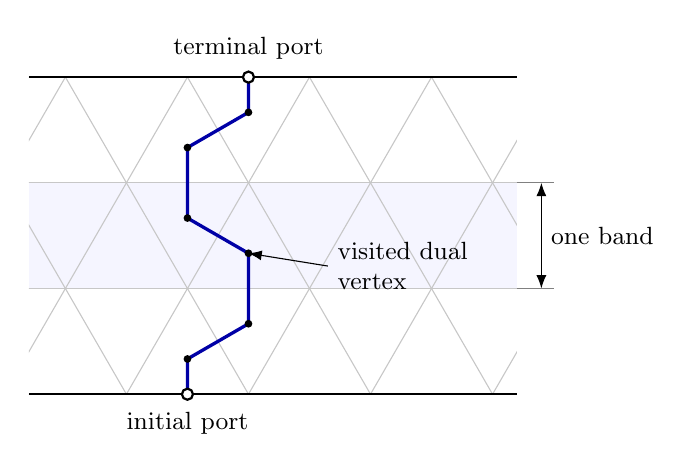
\begin{tikzpicture}[x=1.55cm,y=1.55cm,font=\small,>=Latex]
 \pgfmathsetmacro{\bandheight}{sqrt(3)/2}
 \fill[blue!4] (-.8,\bandheight) rectangle (3.2,2*\bandheight);
 \begin{scope}
  \clip (-.8,0) rectangle (3.2,3*\bandheight);
  \foreach \j in {0,1,2,3}{
   \draw[black!22] (-1,\j*\bandheight)--(4,\j*\bandheight);
  }
  \foreach \j in {0,1,2}{
   \foreach \i in {-3,-2,...,4}{
    \draw[black!22] ({\i+\j/2},\j*\bandheight)
      --({\i+\j/2+.5},{(\j+1)*\bandheight});
    \draw[black!22] ({\i+\j/2},\j*\bandheight)
      --({\i+\j/2-.5},{(\j+1)*\bandheight});
   }
  }
 \end{scope}
 \draw[thick] (-.8,0)--(3.2,0);
 \draw[thick] (-.8,3*\bandheight)--(3.2,3*\bandheight);
 \coordinate (a) at (.5,0);
 \coordinate (v1) at (.5,\bandheight/3);
 \coordinate (v2) at (1,2*\bandheight/3);
 \coordinate (v3) at (1,4*\bandheight/3);
 \coordinate (v4) at (.5,5*\bandheight/3);
 \coordinate (v5) at (.5,7*\bandheight/3);
 \coordinate (v6) at (1,8*\bandheight/3);
 \coordinate (b) at (1,3*\bandheight);
 \draw[very thick,blue!65!black] (a)--(v1)--(v2)--(v3)--(v4)--(v5)--(v6)--(b);
 \foreach \v in {v1,v2,v3,v4,v5,v6}{\fill (\v) circle (1.4pt);}
 \foreach \v in {a,b}{\draw[thick,fill=white] (\v) circle (2pt);}
 \node[below=3pt] at (a) {initial port};
 \node[above=3pt] at (b) {terminal port};
 \node[align=left,anchor=west] (vertex) at (1.65,1.05) {visited dual\\vertex};
 \draw[->] (vertex.west)--(v3);
 \draw[<->] (3.4,\bandheight)--node[right]{one band}(3.4,2*\bandheight);
 \draw[black!50] (3.2,\bandheight)--(3.5,\bandheight);
 \draw[black!50] (3.2,2*\bandheight)--(3.5,2*\bandheight);
\end{tikzpicture}
\caption{Port and length conventions. The path passes through six adjacent
triangles of the triangular tiling, so it visits six vertices of the
honeycomb dual and has port weight $\rho^6$. Its two terminal pieces are
half-edges. An ordinary vertex-to-vertex path counts full edges instead. The shaded region is one triangular band.}
\label{fig:model-conventions}
\end{figure}



\begin{theorem}[Critical strip mass]\label{thm:strip}
For every integer $N\ge1$, all sums in
\eqref{eq:01-strip-quantities} are finite. With constants independent of
$N$,
\begin{equation}\label{eq:01-strip-result}
 c\mathcal A_N+\mathcal B_N=1,\qquad
 m_{N+1}-m_N\asymp\mathcal B_N,\qquad
 m_N\asymp N^{3/4},\qquad
 \mathcal B_N\asymp N^{-1/4}.
\end{equation}
Moreover, $\mathcal B_N$ is nonincreasing in $N$.
\end{theorem}
Here $f_N\asymp g_N$ means that their ratio lies between two fixed
positive constants. Thus the theorem determines a bounded-factor
power law, rather than only a logarithmic exponent. If a height-zero
term is useful, we set $\mathcal B_0=1$ by convention; no strip path is
being added to the definition above. The crossing estimate can then be
written $\mathcal B_N\asymp(1+N)^{-1/4}$ for $N\ge0$.

\subsection{Earlier work}
The two-dimensional polymer exponents arose from the dilute $O(n)$
model and its Coulomb-gas analysis. Nienhuis predicted the honeycomb
critical point and the self-avoiding-walk exponents at
$n=0$~\cite{Nienhuis1982}.
Lawler, Schramm and Werner developed the conjectural conformally
invariant scaling picture for planar self-avoiding walk
\cite[Sections~3.3.1, 3.4.3 and~4.1]{LawlerSchrammWerner2004}.
Their boundary exponent $5/8$ predicts a boundary-to-boundary mass
of power $-5/4$. Summing the endpoint along the opposite side of a
strip then predicts the crossing power $-1/4$; this deduction is
also stated explicitly in \cite[Section~4]{DCS2012}.

Duminil-Copin and Smirnov proved the critical-point prediction using
a parafermionic observable whose local cancellation gives a positive
boundary identity~\cite[Lemmas~1 and~2]{DCS2012}.
Their strip argument gives bounds of order $1/N$ and $1$ for the
crossing mass. These bounds leave the predicted power undetermined.

The decay of this mass was subsequently proved by Beaton,
Bousquet-M\'elou, de Gier, Duminil-Copin and Guttmann in their study of
surface adsorption~\cite[Theorem~10]{BeatonEtAl2014}.
Glazman and Manolescu obtained a shorter proof, a logarithmic bound
along a sequence of heights, and invariance of the half-plane boundary
two-point function under columnwise rhombic deformations with angles
in $[\pi/3,2\pi/3]$
\cite[Proposition~1.1 and Theorems~1--2]{GM2019}.
Krachun and Panagiotis proved a polynomial upper bound
$\mathcal B_N\le100N^{-10^{-10}}$ in their strip convention,
together with quantitative sub-ballisticity
\cite[Theorems~1--2]{KrachunPanagiotis2026}.
Theorem~\ref{thm:strip} establishes the predicted strip power with
uniform multiplicative constants in the port convention above.
The exponent $3/4$ for $m_N$ describes an unnormalized displacement
moment summed over all path lengths, with strip height as its scale.
The fixed-length displacement conjecture and the conjectured conformal
scaling limit concern different observables.

\subsection{Proof strategy}
The boundary identity alone does not determine this power. Our route
is to calculate $m_N$ first and then recover $\mathcal B_N$ from its
increments. The argument passes from finite strip transfers to a
polynomial formula, then to a positive integral that can be estimated
uniformly in the height.

In Section~\ref{sec:flux}, cancellation of closed excursions gives the
boundary identity and controls finite-height transfer matrices. We
introduce rhombic weights with one spectral parameter in each row.
A cut between columns records vacant positions and occupied positions paired
by path pieces on one side of the cut. The stationary vacuum vector
records the weighted sums of these partial pairings with no exterior
source; a source vector has one additional strand connected to a
specified boundary source.
Their local relations belong to the dilute-loop integrable structure;
the relation with discrete parafermions was developed by Ikhlef and
Cardy, and the weighted-walk normalization and corrected general
formulas were treated by Glazman~\cite{IkhlefCardy2009,Glazman2015}.
We prove the exact local identities used here in
Appendix~\ref{app:local-calculations}.

Section~\ref{sec:vacuum} constructs a scalar Pfaffian $p_N$ that turns
the stationary vacuum into a vector of bounded-degree polynomials.
A degree bound is essential: it makes interpolation an identity
argument. Exchange relations and reductions at special parameters
have this role in earlier dense and dilute loop calculations
\cite{DiFrancescoZinnJustin2005,GarbaliNienhuis2017Ground,GarbaliNienhuis2017Sum}.
Here the degree and stationarity arguments are proved for zero loop
weight.
Section~\ref{sec:arch} cuts an arch at every column between its
endpoints. This converts $m_N$ into a pairing of source vectors and
then into one coefficient of $p_{N+1}/p_N$. A stepped-boundary flux
identity proves $m_{N+1}-m_N\asymp\mathcal B_N$.

Section~\ref{sec:integral} converts the homogeneous polynomial problem
into a positive integral over $0<y_1<\cdots<y_N<1$, with density
proportional to
\[
 \prod_{i=1}^N\omega(y_i)
 \prod_{i<j}\frac{(y_j-y_i)^2}{y_i+y_j},\qquad
 \omega(y)=\frac12\sqrt{\sqrt{\frac{1+y}{2y}}-1}.
\]
Positivity of a Cauchy-moment determinant makes the coincident-parameter
limit nonsingular.
The pair interaction in the resulting integral is the one appearing in
generalized Bures ensembles~\cite{ForresterKieburg2016}.
The derivation from the strip polynomial fixes the normalization and
identifies the integral with the arch moment. Finally,
Section~\ref{sec:hard-edge} compares this measure with Bures--Laguerre
laws. Schur's Pfaffian identity and de Bruijn's integration formula
give their normalizing constants; positive association gives the
comparison. The smallest-coordinate estimates yield
$m_N\asymp N^{3/4}$. Monotonicity and the increment identity then give
the crossing power in Theorem~\ref{thm:strip}.

\section{Positive flux and finite strip transfers}\label{sec:flux}

We write
\begin{equation}\label{eq:01-constants}
 t=\frac38,\qquad \lambda=\frac\pi8,\qquad
 d=\cos(2\lambda)=\sin(2\lambda),\qquad C=\cos\lambda.
\end{equation}
Then $c=\cos(3\lambda)$ and $\rho=C-c=1/(2C)$, consistently
with \eqref{eq:critical-weight}.

The boundary identity controls positive path sums before any spectral parameter is introduced. We use it first to make the fixed-height transfer construction convergent. The local identities then allow the stationary vector to be recovered by polynomial interpolation.


\begin{lemma}[Boundary identity]\label{lem:boundary-flux}
Let $D$ be a finite simply connected union of triangles with simple
polygonal boundary, and let $a$ be a boundary port. If $W(\gamma)$ is
the total signed turning of a path, measured from its inward initial
direction to its outward final direction, then
\begin{equation}\label{eq:01-boundary-identity}
 \sum_{b\in\partial D}\ \sum_{\gamma:a\to b}
       \rho^{|\gamma|}e^{itW(\gamma)}=1.
\end{equation}
If $D$ is convex, its unsigned boundary partition sum is at most $1/c$.
\end{lemma}

\begin{proof}
Send mass one along the inward half-edge at $a$. At each newly visited
vertex split it between the two possible continuations, multiplying by
$\rho e^{i\lambda}$ and $\rho e^{-i\lambda}$, respectively. The identity
$2\rho\cos\lambda=1$ conserves total mass. Stop a branch when it exits
$D$ or is about to enter a vertex already visited. This produces a finite
tree because $D$ has finitely many vertices.

For a stopped collision, the newly closed cycle is simple and has a
disjoint incoming stem. The stem lies outside the cycle: it starts on
$\partial D$ and cannot cross the cycle before their first common
vertex. Consequently the unused branch at that vertex is exterior to
the cycle. The cycle turn there is $\pi/3$ in the counterclockwise
orientation, rather than $-\pi/3$; the clockwise statement is reversed.
The turn from the stem into the cycle replaces this closing turn by its
negative. The two ways to traverse the cycle therefore have winding
increments $4\pi/3$ and $-4\pi/3$ relative to the stem. They have the
same unsigned weight and cancel, since
$e^{it(4\pi/3)}+e^{-it(4\pi/3)}=0$. Cycle reversal is an involution on
all stopped collisions. The remaining terminal mass gives
\eqref{eq:01-boundary-identity}.

For a path ending at $b$, close it using the counterclockwise boundary
arc from $b$ to $a$. The turns at the two ports are $\pi/2$, so the
turning theorem for this simple closed curve gives
\[
 W(\gamma)=\pi-\operatorname{turn}_{\partial D}(b\to a).
\]
For a convex boundary the latter turn lies in $[0,2\pi]$. Thus
$|W(\gamma)|\le\pi$ and
$\cos(tW(\gamma))\ge\cos(3\pi/8)=c$.
Taking real parts proves the last assertion.
\end{proof}

We next introduce auxiliary spectral parameters. A column has $N$
rhombi stacked along horizontal edges; in row $i$ the other edge makes
angle $u_i/t$ with the horizontal. The same tiles make sense as
combinatorial diagrams for complex $u_i$. Their four ports carry
noncrossing partial pairings. Port occupancies must agree when tiles
are glued, and every closed component has weight zero. Put
\begin{equation}\label{eq:01-rhombic-weights}
\begin{aligned}
 a(u)&=\cos(2u-3\lambda),&
 L(u)&=\sin(2\lambda+u)\sin(3\lambda+u)=\frac{C+a(u)}2,\\
 A(u)&=\frac{d\sin(3\lambda-u)}{L(u)},&
 U(u)&=\frac{d\sin u}{L(u)},\\
 B(u)&=\frac{\sin u\sin(3\lambda-u)}{L(u)}
       =\frac{a(u)-c}{a(u)+C},\\
 E(u)&=\frac{\sin(3\lambda-u)\sin(2\lambda-u)}{L(u)},&
 F(u)&=\frac{\sin(u-\lambda)\sin u}{L(u)}.
\end{aligned}
\end{equation}
These weights come from Nienhuis's integrable $O(n)$ construction
\cite{Nienhuis1990CriticalMulticritical}, in the self-avoiding-walk
normalization displayed in \cite{GM2019}; the general parafermionic and integrable local formulas
are discussed in \cite{IkhlefCardy2009,Glazman2015}.
The empty tile has weight one. A single connection between opposite
ports has weight $B$. A bottom--left or top--right turn has weight $A$;
the other two turns have weight $U$. The configurations with two turns
of the first or second type have weights $E$ and $F$, respectively.
At $u=\lambda$ or $2\lambda$, splitting along the short diagonal recovers
two triangular tiles, with weight $\rho$ per visited triangle. At
$u=0$ or $3\lambda$ the row is flat: each route continues deterministically
through the adjacent left or right port, and the two disjoint routes
can coexist with weight one.

The dilute diagram algebra and its Yang--Baxter operators have an
algebraic construction in Grimm and Pearce~\cite{GrimmPearce1993}.
Their distinction between gauge-invariant periodic partition functions
and other gauge-dependent quantities is relevant here: we specify the caps, scalar factors
and port ordering, and prove the identities for these choices.

We use the planar diagram algebra whose inputs and outputs are ordered
slots, each vacant or occupied. Composition glues matching slots and
annihilates a mismatch or a closed loop. Tensor product means
juxtaposition; transpose reflects a diagram, interchanging inputs and
outputs. The two-slot operator $R(v)$ has coefficients
$1,A(v),B(v),U(v),E(v),F(v)$ on, respectively, the empty diagram, a
single vertical connection, a single diagonal connection, a cap alone
or cup alone, two vertical connections, and a cap together with a cup.
There are two choices for a single vertical or diagonal connection, as
shown in Figure~\ref{fig:local-operator}.

\begin{figure}[htbp]
\centering
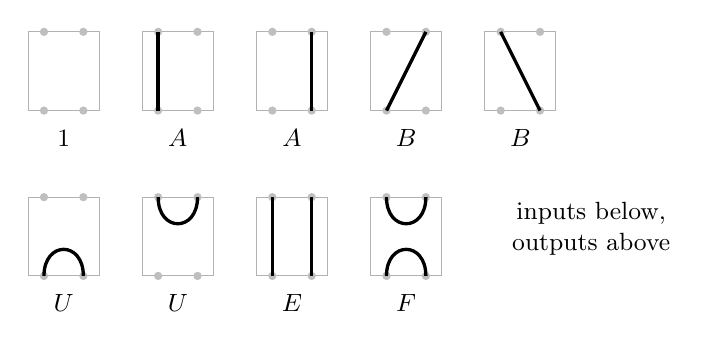
\begin{tikzpicture}[x=1cm,y=1cm,font=\small]
\foreach \j/\wt in {0/1,1/A,2/A,3/B,4/B,5/U,6/U,7/E,8/F}{
 \begin{scope}[xshift={1.45*mod(\j,5)*1cm},yshift={-2.1*floor(\j/5)*1cm}]
 \draw[black!30] (-.45,0) rectangle (.45,1);
 \foreach \x in {-.25,.25}{\fill[black!25] (\x,0) circle (1.5pt);\fill[black!25] (\x,1) circle (1.5pt);}
 \ifnum\j=1 \draw[very thick] (-.25,0)--(-.25,1);\fi
 \ifnum\j=2 \draw[very thick] (.25,0)--(.25,1);\fi
 \ifnum\j=3 \draw[very thick] (-.25,0)--(.25,1);\fi
 \ifnum\j=4 \draw[very thick] (.25,0)--(-.25,1);\fi
 \ifnum\j=5 \draw[very thick] (-.25,0) .. controls (-.25,.45) and (.25,.45) .. (.25,0);\fi
 \ifnum\j=6 \draw[very thick] (-.25,1) .. controls (-.25,.55) and (.25,.55) .. (.25,1);\fi
 \ifnum\j=7 \draw[very thick] (-.25,0)--(-.25,1) (.25,0)--(.25,1);\fi
 \ifnum\j=8 \draw[very thick] (-.25,0) .. controls (-.25,.45) and (.25,.45) .. (.25,0);\draw[very thick] (-.25,1) .. controls (-.25,.55) and (.25,.55) .. (.25,1);\fi
 \node at (0,-.35) {$\wt$};
 \end{scope}
}
\node[align=center] at (6.7,-1.5) {inputs below,\\outputs above};
\end{tikzpicture}
\caption{The nine local diagrams of $R(v)$, with coefficients evaluated
at $v$. Grey dots mark available slots; a slot is occupied exactly when a
black strand meets it. Gluing requires matching occupancies and assigns
zero to every closed component. These are operator diagrams, rather than
a geometric drawing of a rhombus.}
\label{fig:local-operator}
\end{figure}


Number the rows from bottom to top. A column swept from left to right
uses $R(3\lambda-u_i)$ in row $i$, with local ordered inputs
(south, west) and outputs (east, north). The north output of row $i$
is the south input of row $i+1$. The geometric and operator weights agree
because
\[
 A(3\lambda-u)=U(u),\quad U(3\lambda-u)=A(u),\quad
 B(3\lambda-u)=B(u),\quad E(3\lambda-u)=F(u).
\]
The last relation also gives $F(3\lambda-u)=E(u)$.
Figure~\ref{fig:rhombus-dictionary} records the port order.

\begin{figure}[htbp]
\centering
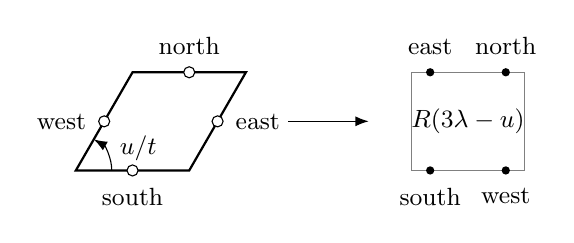
\begin{tikzpicture}[x=1.2cm,y=1.2cm,font=\small,>=Latex]
 \draw[thick] (0,0)--(1.2,0)--(1.8,1.039)--(.6,1.039)--cycle;
 \foreach \x/\y/\label/\pos in {.6/0/south/below,.3/.5195/west/left,1.5/.5195/east/right,1.2/1.039/north/above}{
  \draw[fill=white] (\x,\y) circle (2pt);
  \node[\pos=3pt] at (\x,\y) {\label};
 }
 \draw[->] (.38,0) arc[start angle=0,end angle=60,radius=.38];
 \node at (.66,.23) {$u/t$};
 \draw[->] (2.25,.52)--(3.1,.52);
 \draw[black!50] (3.55,0) rectangle (4.75,1.039);
 \node at (4.15,.52) {$R(3\lambda-u)$};
 \foreach \x/\y/\label/\pos in {3.75/0/south/below,4.55/0/west/below,3.75/1.039/east/above,4.55/1.039/north/above}{
  \fill (\x,\y) circle (1.5pt);
  \node[\pos=3pt] at (\x,\y) {\label};
 }
\end{tikzpicture}
\caption{From a geometric rhombus to a column operator. South and west
are the ordered inputs; east and north are the ordered outputs. The
operator is drawn with its inputs below and outputs above, so the
rhombic parameter $u$ corresponds to the operator argument $3\lambda-u$.
The rhombus is schematic; only the angle label and port order matter.}
\label{fig:rhombus-dictionary}
\end{figure}



Define $S_2$, from one slot to two, by sending a vacancy to a vacancy
plus $\rho$ times a cup, and an occupied strand to either output slot
with coefficient $\rho$. Define $S_3$, from no slots to two, to be the
sum of the vacant diagram and a cup.

\begin{lemma}[Local diagram identities]\label{lem:local-identities}
Writing $R_i$ for action in slots $i,i+1$, one has
\begin{align}
 R_2(y)R_1(x+y)R_2(x)&=R_1(x)R_2(x+y)R_1(y),
       \label{eq:01-braid}\\
 R(s\lambda)&=S_sS_s^{\mathsf t},\qquad s=2,3,
       \label{eq:01-factorization}\\
 R_2(x)R_1(x+s\lambda)(I\otimes S_s)
       &=(S_s\otimes I)\widehat R_s(x),
       \label{eq:01-splitting}\\
 R(x)R(-x)&=I.\label{eq:01-unitarity}
\end{align}
Here $\widehat R_2(x)=R(x+\lambda)$ and $\widehat R_3(x)$ is the
one-slot identity. These are identities of rational functions. They
can be specialized wherever the relevant sides are regular, including
at removable singularities; an individual operator at a genuine pole
is not assigned a finite value.
\end{lemma}

The complete coefficient proof is in Appendix~\ref{app:local-calculations}.


For a cut between two columns of $N$ rows, number its slots from
bottom to top. Let $\mathcal L_N^0$ be the vector space with basis the
noncrossing partial pairings of occupied slots; all other slots are
vacant. Let $\mathcal L_N^1$ have the same pairings with one additional
unpaired occupied slot connected to an exterior source. This defect
cannot be enclosed by a pair. Restricting a single path to one side
of a cut can produce several paired fragments as well as the
source-connected strand, as Figure~\ref{fig:cut-states} illustrates.

\begin{figure}[htbp]
\centering
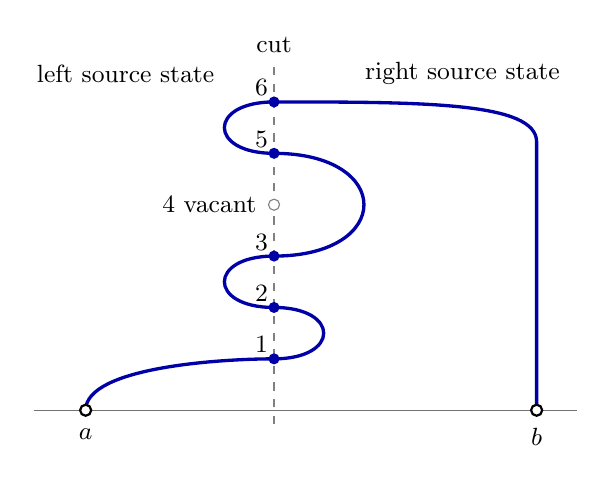
\begin{tikzpicture}[x=1.45cm,y=1.45cm,font=\small,>=Latex]
 \draw[black!55] (-2.1,0)--(2.65,0);
 \draw[dashed,black!50] (0,-.12)--(0,3.05);
 \node[above] at (0,3.05) {cut};
 \node at (-1.3,2.95) {left source state};
 \node at (1.65,2.95) {right source state};
 \draw[very thick,blue!65!black]
   (-1.65,0) .. controls (-1.65,.38) and (-.45,.45) .. (0,.45)
   .. controls (.58,.45) and (.58,.9) .. (0,.9)
   .. controls (-.58,.9) and (-.58,1.35) .. (0,1.35)
   .. controls (1.05,1.35) and (1.05,2.25) .. (0,2.25)
   .. controls (-.58,2.25) and (-.58,2.7) .. (0,2.7)
   .. controls (1.3,2.7) and (2.3,2.7) .. (2.3,2.35)
   -- (2.3,0);
 \foreach \j/\y in {1/.45,2/.9,3/1.35,5/2.25,6/2.7}{
  \fill[blue!65!black] (0,\y) circle (2pt);
  \node[anchor=south east,inner sep=2pt] at (0,\y) {$\j$};
 }
 \draw[black!50,fill=white] (0,1.8) circle (2pt);
 \node[anchor=east] at (-.07,1.8) {$4$ vacant};
 \draw[thick,fill=white] (-1.65,0) circle (2pt);
 \draw[thick,fill=white] (2.3,0) circle (2pt);
 \node[below=3pt] at (-1.65,0) {$a$};
 \node[below=3pt] at (2.3,0) {$b$};
\end{tikzpicture}
\caption{A single arch may cross a cut several times. In this schematic
example the left half has a source strand at slot $1$ and pairs $(2,3)$,
$(5,6)$; the right half has pairs $(1,2)$, $(3,5)$ and a source strand
at slot $6$. Slot $4$ is vacant on both sides. Each source strand is
exposed, meaning that no pair encloses its slot. Gluing the two states
recovers one path from $a$ to $b$, with no closed component.}
\label{fig:cut-states}
\end{figure}


Before fixing its two auxiliary ends, the complete column is the map
\begin{equation}\label{eq:full-column}
 M_X=R_N(v_N)\cdots R_1(v_1),\qquad
 v_i=3\lambda-u_i,\qquad X=(u_1,\ldots,u_N).
\end{equation}
Its ordered inputs are $(\mathrm{aux},1,\ldots,N)$ and its ordered
outputs are $(1,\ldots,N,\mathrm{aux})$: the auxiliary slot moves from
the south end to the north end of the column. Attach a cut state to
the west inputs, glue matching occupancies, and record the east state,
assigning zero to any closed loop. With both auxiliary ends vacant,
this defines $T_N^{(\epsilon)}:\mathcal L_N^\epsilon\to
\mathcal L_N^\epsilon$, $\epsilon=0,1$; write $T_N=T_N^{(0)}$.
With the south end occupied and the north end vacant, it defines the
source insertion $\mathsf b_N:\mathcal L_N^0\to\mathcal L_N^1$.
Interchanging these end conditions defines $\mathsf b_N^{\rm north}$.
A superscript $-$ denotes the corresponding maps for a sweep from
right to left. Horizontal reflection replaces $X$ by
$X^*=(3\lambda-u_1,\ldots,3\lambda-u_N)$, so its complete column is
$M_X^-=R_N(u_N)\cdots R_1(u_1)$.
The empty coordinate of $T_Nv$ equals that of $v$: any occupied input
that closed up before reaching an output would form a forbidden loop.

\noindent\begin{minipage}{\linewidth}
\begin{lemma}[Decay and rational continuation]\label{lem:transfer-decay}
If every $u_i$ belongs to $\{0,\lambda,2\lambda,3\lambda\}$, then
$T_N$ restricted to vectors with zero empty coordinate and
$T_N^{(1)}$ have spectral radius strictly less than one. The same
holds for reversed columns and in a complex neighborhood of each
such parameter list, with absolute values of tile weights used to
control absolute convergence.

There is consequently a unique stationary vacuum vector $P_N$ with
empty coordinate one. Its entries are rational in the $e^{iu_i}$,
and regular at every parameter list just specified.
\end{lemma}
\end{minipage}\par

\begin{proof}
First take a homogeneous triangular parallelogram of height $H>0$
and width $M$. The total weight of paths from a fixed left port to
its right side tends to zero as $M\to\infty$. To see this, append a
column immediately to the right of the exit and continue, entirely
inside this new column, to its bottom port. The continuation has at most a fixed number
of vertices depending only on $H$, so its weight is bounded below
by a positive constant depending only on $H$. For every $M<L$ these
extensions are paths in a parallelogram of width $L$. Their bottom
endpoints identify $M$, and their first exit into the appended
column recovers the original path. They are therefore distinct.
Writing $q_H(M)$ for the crossing mass and $C_H$ for the maximum
number of added vertices, Lemma~\ref{lem:boundary-flux} gives
\[
 \rho^{C_H}\sum_{M<L}q_H(M)\le 1/c.
\]
Thus $q_H(M)\to0$. The same lemma uniformly bounds paths joining
ports on the same side.

For a mixed list of the four allowed parameters, collapse the flat
rows. The row vectors belong to
$\{1,e^{i\pi/3},e^{2i\pi/3},-1\}$, so outside two end pieces of
horizontal size $O(N)$ the remaining triangles form a homogeneous
parallelogram of height $H$, the number of nonflat rows, and width
$M-O(N)$. This description does not depend on which neighboring
triangles were grouped into rhombi. A collapsed deterministic route
drifts by at most $N$ columns. The end pieces have bounded size for
fixed $N$ and contribute bounded weights.

Every nonzero diagram contributing to either restricted transfer
power has a component connecting the left and right cuts. In the
vacuum sector, otherwise the nonempty input pairing would close
into a loop; in the source sector, the source must reach the output.
Cut all components at the two ends of the homogeneous core. There
are only boundedly many endpoint patterns, depending on $N$, and at
least one segment spans the core. Ignoring avoidance between these
segments bounds their total weight by a product of single-path
partition sums. Each nonspanning factor is at most $1/c$.
For $H>0$, choose the core width $M-\kappa_X$, where the fixed
offset satisfies $0\le\kappa_X=O(N)$. If $Q_N$ is the nonempty vacuum block and
$\|\cdot\|_{\max}$ is the maximum absolute matrix entry, then
\[
 \|Q_N^M\|_{\max}+\|(T_N^{(1)})^M\|_{\max}
 \le C_N\sum_{a\in\mathcal E_H}q_{H,a}(M-\kappa_X)\longrightarrow0.
\]
Here $\mathcal E_H$ is the finite set of left ports of the core,
$q_{H,a}$ is its crossing mass from $a$, and $C_N$ absorbs the bounded
end pieces and endpoint patterns. All constants are for fixed $N$;
no uniform spectral gap is needed. If $H=0$,
no spanning component is possible once $M$ is sufficiently large.
Thus both restricted matrix powers tend to zero. Since these are
finite matrices, their spectral radii are less than one.

At the specified parameters all tile weights are nonnegative. The
matrices obtained by taking absolute tile weights vary continuously,
so their restricted spectral radii remain less than one in a small
complex neighborhood. This also proves the asserted absolute
convergence. The reflected argument is identical.

Writing the vacuum matrix in the empty/nonempty decomposition gives
$T_N=\left(\begin{smallmatrix}1&0\\v&Q\end{smallmatrix}\right)$.
Its normalized stationary vector is $(1,(I-Q)^{-1}v)$, which is regular
in the stated neighborhoods and rational in the spectral variables.
This proves both uniqueness and the continuation claim. Equivalently,
$P_N$ is the sum of finite path diagrams in the vacuum half-strip.
\end{proof}

We now pass from local identities to column identities. This also
records the source insertions needed for the arch moment. Let $X'$ be
$X$ with adjacent rows $i,i+1$ exchanged, and put
$\delta=u_{i+1}-u_i$. Applying the braid relation to those rows gives
\begin{equation}\label{eq:column-exchange}
 M_X(I_{\rm aux}\otimes R_i(\delta))
 =(R_i(\delta)\otimes I_{\rm aux})M_{X'}.
\end{equation}
The tensor positions reflect the different input and output orders
in \eqref{eq:full-column}.
If $u_{i+1}=u_i+s\lambda$, $s=2,3$, let $X_{\rm red}$ replace these
rows by $u_i+\lambda$ for $s=2$, or delete them for $s=3$.
The splitter $S_s$ acts on these cut slots, with identities on all
other slots. In each sector it maps
$\mathcal L_{N-r_s}^\epsilon$ to $\mathcal L_N^\epsilon$, where
$r_2=1$ and $r_3=2$. The local splitting identity yields
\begin{equation}\label{eq:column-splitting}
 M_X(I_{\rm aux}\otimes S_s)
 =(S_s\otimes I_{\rm aux})M_{X_{\rm red}}.
\end{equation}
Indeed its argument is $x=v_{i+1}$, and for $s=2$ the effective box
has argument $x+\lambda=3\lambda-(u_i+\lambda)$, as required.
Transpose splitting and reverse the slot order to obtain the reflected
projection identity
\begin{equation}\label{eq:column-reflection}
 (S_s^{\mathsf t}\otimes I_{\rm aux})M_X^-
 =M_{X_{\rm red}}^-(I_{\rm aux}\otimes S_s^{\mathsf t}).
\end{equation}
All three equations leave the auxiliary endpoints untouched. We can
therefore impose either vacant ends or either source-insertion
condition. With $X$ as a subscript denoting its row list, this gives,
for $\epsilon=0,1$,
\begin{equation}\label{eq:transfer-intertwiners}
\begin{aligned}
 T_X^{(\epsilon)}R_i(\delta)&=R_i(\delta)T_{X'}^{(\epsilon)},&
 \mathsf b_XR_i(\delta)&=R_i(\delta)\mathsf b_{X'},\\
 T_X^{(\epsilon)}S_s&=S_sT_{X_{\rm red}}^{(\epsilon)},&
 \mathsf b_XS_s&=S_s\mathsf b_{X_{\rm red}},\\
 S_s^{\mathsf t}T_X^{(\epsilon),-}
 &=T_{X_{\rm red}}^{(\epsilon),-}S_s^{\mathsf t},&
 S_s^{\mathsf t}\mathsf b_X^-
 &=\mathsf b_{X_{\rm red}}^-S_s^{\mathsf t}.
\end{aligned}
\end{equation}
The same equations hold with $\mathsf b^{\rm north}$ in place of
$\mathsf b$. In a source-insertion equation the cut map on its right
acts in the vacuum sector and the cut map on its left acts in the
one-source sector.

The normalized stationary vector is now determined under exchange
and reduction:
\begin{align}
 P_N(\ldots,u_i,u_{i+1},\ldots)
 &=R_i(u_{i+1}-u_i)P_N(\ldots,u_{i+1},u_i,\ldots),
 \label{eq:01-vacuum-exchange}\\
 P_N&=S_sP_{\mathrm{red}}
 \quad\text{when }u_{i+1}=u_i+s\lambda.
 \label{eq:01-vacuum-reduction}
\end{align}
The column equations prove stationarity of the right sides. Their empty
coordinate is one: a cap producing an empty output from a nonempty
pairing would close a zero-weight loop. Uniqueness in
Lemma~\ref{lem:transfer-decay} proves exchange near the all-zero
parameter list, and reduction near a mixed list with $u_i=0$.
Intersecting these regular neighborhoods with the specialization
hypersurface gives an open set in that hypersurface. Rational
continuation then proves the identities for general parameters.
The reflected projection and source equations will be used in the
same way, with uniqueness of the corresponding stationary or
inhomogeneous transfer equation.

At $u_1=3\lambda$, the first slot is vacant and can be deleted. At
$u_1=0$, the part with first slot vacant is $P_{N-1}$; the occupied
part is obtained from $P_{N-1}$ by one column on rows $2,\ldots,N$
with a south source and vacant north, tying that source to slot $1$.
These assertions follow from $R(0)=I$ and
$R(3\lambda)=S_3S_3^{\mathsf t}$; in the latter identity an occupied
first input with vacant auxiliary input contributes zero.
Finally, shifting $u_k$ by $\pi$ multiplies each tile weight by the
occupancy signs at its west and east ports. Thus it conjugates $T_N$
by the diagonal map $D_k$ that changes the sign of states with slot
$k$ occupied. Since $D_k$ preserves the empty coordinate, uniqueness
gives $P_N(X+\pi e_k)=D_kP_N(X)$, where $e_k$ is the $k$th coordinate
vector.

\section{The polynomial vacuum}\label{sec:vacuum}

The stationary vacuum is initially only a rational vector. To extract a physical observable at coincident parameters, we need a polynomial numerator with a controlled degree. We first construct its scalar normalization and then prove the vector degree bound by interpolation and stationarity.


Exchange equations, degree bounds and reductions at special rapidities
have earlier uses in the dense $O(1)$ model
\cite{DiFrancescoZinnJustin2005} and in the open dilute $O(1)$ model
\cite{GarbaliNienhuis2017Ground,GarbaliNienhuis2017Sum}.
The latter comparison concerns the fusion construction of the polynomial
normalization. A related verification of a Pfaffian normalization by
deletion identities and degree bounds appears for the crossing $O(1)$
model in \cite[Section~2.6]{DiFrancesco2005Open}.
We construct the present zero-loop-value scalar and vector
with their own degree and stationarity proofs.

Write $X=(u_1,\ldots,u_N)$ and $a_i=a(u_i)$. Define
\begin{equation}\label{eq:01-pfaffian}
\begin{split}
 D(a,b)&=a^2+b^2+2dab-d^2,\\
 p_N(a_1,\ldots,a_N)
 &=\prod_{i<j}\frac{D(a_i,a_j)}{a_i-a_j}
   \operatorname{Pf}\left[
    \frac{(a_i-a_j)(a_i+a_j+\rho)}{D(a_i,a_j)}
   \right].
\end{split}
\end{equation}
For odd $N$, augment the skew matrix by a last column of ones and its
negative transpose; set $p_0=1$.

\begin{lemma}[Scalar reduction identities]\label{lem:scalar-reductions}
The function $p_N$ is a symmetric polynomial of degree at most $N-1$
in each argument. Its leading coefficient in any argument is
$p_{N-1}$ of the remaining arguments, and
\begin{equation}\label{eq:01-scalar-flat}
 p_N(Y,c)=p_{N-1}(Y)\prod_{z\in Y}(z+C).
\end{equation}
For $f_j=\cos(w+j\lambda)$,
\begin{align}
 p(Y,f_0,f_6)
 &=p(Y)(f_0+f_6+\rho)
       \prod_{z\in Y}(z-f_{-6})(z-f_{12}),
       \label{eq:01-scalar-delete}\\
 p(Y,f_{-2},f_2)
 &=p(Y,f_0)(f_{-2}+f_2+\rho)
       \prod_{z\in Y}(z+f_0).
       \label{eq:01-scalar-merge}
\end{align}
Here the subscript of $p$ is its number of arguments. Both formulas
also hold with all shifts negated.
\end{lemma}

\begin{proof}
After multiplication by all $D$ factors, the Pfaffian is an alternating
polynomial, hence divisible by the Vandermonde product in
\eqref{eq:01-pfaffian}. Counting degrees before and after division
gives degree at most $N-1$ in each variable. Letting a last argument
tend to infinity proves the leading-coefficient statement: its kernel
entries tend to $-1$. In odd size first add the augmenting column and
row to that argument's column and row. At the flat value,
$D(z,c)=(z-c)(z+C)$ and the kernel entry equals one. This proves
\eqref{eq:01-scalar-flat}.

At $D(f_0,f_6)=0$ only Pfaffian terms pairing these two arguments
survive after denominators are cleared. The identity
$D(f_0,z)=(z-f_{-6})(z-f_6)$ then gives
\eqref{eq:01-scalar-delete}.

Prove the merge identity by induction on $r=|Y|$. The case $r=0$
follows from $p_2(a,b)=a+b+\rho$. If $r\ge1$, distinguish a spectator
$z$. Both sides have degree at most $r+1$ in $z$, and their leading
coefficients agree by induction. They vanish at $z=-f_0$: delete
this argument with $f_{-2}$, and the remaining factor involving
$f_2$ vanishes. At $z=c$ they agree by the flat formula and
\[
 (C+f_{-2})(C+f_2)=(c+f_0)(C+f_0).
\]
They also agree at each deletion value of $z$ with another spectator.
To check the factors, write that pair as $g_0,g_6$, where
$g_j=\cos(v+j\lambda)$, and use
\[
 \prod_{\ell=\pm2}(f_\ell-g_{-6})(f_\ell-g_{12})
 =(f_0+g_0)(f_0+g_6)(f_0-g_{-6})(f_0-g_{12}).
\]
This is the product-to-sum identity obtained from shifts by
$\pm2\lambda$. There are $2(r-1)$ such deletion values, in addition
to $-f_0$ and $c$. For generic arguments these are distinct and give
at least $r+1$ roots for a difference of degree at most $r$, after
its leading coefficient has canceled. Polynomial continuation concludes
the proof.
\end{proof}

\begin{lemma}[Vacuum degree bound]\label{lem:vacuum-degree}
The vector $W_N=p_NP_N$ is Laurent polynomial in $e^{iu_1},\ldots,e^{iu_N}$,
with each exponent between $-(2N-2)$ and $2N-2$. In the last variable
$y=u_N$, $b=a(y)$, its last-slot-vacant part is a polynomial in $b$
of degree at most $N-1$ with leading coefficient $W_{N-1}$.
Its last-slot-occupied part is $\sin y$ times a polynomial in $b$ of
degree at most $N-2$. Set $W_0=1$.
\end{lemma}

\begin{proof}
The assertion for $N=1$ is immediate. We construct the asserted
polynomial by induction and then prove its stationarity. Throughout the
construction, $W$ denotes the candidate at size $N$, whereas every
smaller $W_j=p_jP_j$ is already known by induction. We first remove
the candidate's possible poles and bound its degree, then establish
its special-row relations, and finally use those relations to prove
stationarity.

Deleting a vacant last slot identifies that sector with
$\mathcal L_{N-1}^0$. Deleting an occupied last slot leaves its partner
as the exposed defect of a state in $\mathcal L_{N-1}^1$. We use these
identifications for the subscripts $v$ and $o$ below.

\paragraph{Construction and regularity.}

For each earlier row $i<N$, introduce the deletion node and its
associated cosine values
\[
 y_i=u_i+3\lambda,\quad \beta_i=a(y_i),\quad
 \gamma_i=a(u_i-3\lambda),\quad \sigma_i=a(u_i+6\lambda).
\]
Let $\mathcal R_i$ move the newly inserted row $y_i$ from immediately
above row $i$ to the last position, using successive boxes with
arguments $y_i-u_j$, $i<j<N$. By
\eqref{eq:01-vacuum-exchange}, \eqref{eq:01-vacuum-reduction}, and
\eqref{eq:01-scalar-delete}, the value required at $y=y_i$ is
\begin{equation}\label{eq:01-interpolation-data}
 Y_i=(a_i+\beta_i+\rho)
       \prod_{\substack{j<N\\j\ne i}}
           (a_j-\gamma_i)(a_j-\sigma_i)\,
       \mathcal R_i S_3W_{N-2}(X\setminus\{u_i,u_N\}).
\end{equation}
These data agree with the genuine rational vector $p_NP_N$ on the
node hypersurface: one may check the identity near $u_i=0$ with the
other rows mixed, where all stationary vectors are regular. The mixed point supplies an
open neighborhood within the hypersurface, so this establishes a rational
identity in the remaining parameters, not just equality at one point.

For distinct nodes put
\[
 \ell_i(b)=\prod_{\substack{j<N\\j\ne i}}
                 \frac{b-\beta_j}{\beta_i-\beta_j}.
\]
Define the candidate by the two interpolation formulas
\begin{equation}\label{eq:vacuum-interpolants}
 \begin{aligned}
 W_v(b)&=W_{N-1}\prod_{i<N}(b-\beta_i)
                 +\sum_{i<N}(Y_i)_v\ell_i(b),\\
 W_o(y)&=\sin y\sum_{i<N}\frac{(Y_i)_o}{\sin y_i}\ell_i(b).
 \end{aligned}
\end{equation}
The vacant part has degree at most $N-1$ and leading coefficient
$W_{N-1}$; the occupied part divided by $\sin y$ has degree at most
$N-2$. Both have the prescribed node values. Scalar interpolation
shows that the empty coordinate of $W$ is $p_N$.

We check carefully that this construction has no poles in earlier
spectral variables. Each moving box has two sine factors in its
denominator; they divide the factors
$(a_j-\gamma_i)(a_j-\sigma_i)$ in
\eqref{eq:01-interpolation-data}. The possible divisor $\sin y_i$
in the occupied data also cancels. Explicitly, for $x=u_i$ and
$v=u_j$, the two cancellations are
\[
 \frac{(a(v)-a(x-3\lambda))(a(v)-a(x+6\lambda))}{L(x+3\lambda-v)}
 =-4\sin(x+v-6\lambda)\sin(x+v+3\lambda),
\]
\[
 a(x)+a(x+3\lambda)+\rho
 =4c\sin(x+3\lambda)\sin(3\lambda-x).
\]
The remaining possible divisors come from colliding interpolation
nodes. Since
\[
 \beta_i-\beta_j
 =-2\sin(u_i+u_j+3\lambda)\sin(u_i-u_j),
\]
the two components of $\beta_i=\beta_j$ are
\[
 u_i=u_j\pmod\pi,
 \qquad u_i+u_j=-3\lambda\pmod\pi.
\]
On the first component the data, including the divided occupied data,
agree by their identities with the true vector and its occupancy
signs. This can be verified near the regular mixture
$u_i=u_j=0$, $y_i=y_j=3\lambda$. On the second component both data
vanish through their factors involving $\sigma_i,\sigma_j$; at a
generic point no moving-box denominator vanishes. These checks at
generic points of every irreducible divisor suffice, since all
possible denominators are products of the indicated simple Laurent
factors. Thus $W$ is Laurent polynomial in the earlier variables;
multiple intersections of these divisors introduce no further denominators.

For its degree, send an earlier $u_k$ to either Laurent extreme.
The moving boxes remain bounded there, as follows directly from
the weights in \eqref{eq:01-rhombic-weights}.
Data with $i\ne k$ grow at most like $a_k^{N-1}$: they contain two
scalar factors and the inductive vector $W_{N-2}$, while
$\ell_i(b)$ stays bounded. Data with $i=k$
grow at most like $a_k^{1+2(N-2)}$, while their Lagrange cardinal
polynomial contributes $O(a_k^{-(N-2)})$. The leading-coefficient
term $W_{N-1}\prod_{i<N}(b-\beta_i)$ has the same bound. Since poles
have already been removed, growth at the two Laurent extremes bounds
every earlier exponent between $-(2N-2)$ and $2N-2$. Interpolation preserves
the occupancy sign under a shift $u_k\mapsto u_k+\pi$; when the
shift affects a node, its last-slot sign cancels the sign of the
dividing sine.

\paragraph{Relations in the earlier rows.}
Earlier-row braid covariance follows from the same last-variable
interpolation: the exchange box is independent of the last variable,
the leading coefficients agree by induction, and every node datum agrees
by the rational vacuum exchange identity. Uniqueness of the interpolant
then gives covariance.

We have established the degree bounds and prescribed node values of
$W$. To prove stationarity, we need more zeros than the last-variable
interpolation supplies. The next two row specializations provide those
zeros; the final argument combines them with the degree bounds and
occupancy parity. Both specializations are proved by interpolation in
the last variable.
\begin{enumerate}
\item If adjacent earlier rows satisfy $u_{r+1}=u_r+s\lambda$,
$s=2,3$, the interpolant equals the smaller split vector multiplied
by the corresponding scalar quotient from
\eqref{eq:01-scalar-delete} or \eqref{eq:01-scalar-merge}.
The quotient has degree one in $b$ for merge and two for deletion,
with monic last-variable factor. Thus the required degree forms and leading
coefficient agree by induction. At a node indexed by $i\ne r+1$,
compare both expressions with the true vector near a regular
simultaneous specialization: take $u_r=0$, $u_i=0$ when distinct,
and $y_i=3\lambda$, with the other rows mixed. At $i=r+1$ both
expressions vanish. On the split side the vanishing factor is
$b-\sigma_r$ in deletion or $b+a(u_r+\lambda)$ in merge. On the
node-data side it is $a_r-\gamma_i$ or $a_r-\sigma_i$, respectively;
no moving box crosses row $r$. This proves the specialization.
\item At $u_1=0$ or $3\lambda$, use the first-slot formulas following
\eqref{eq:01-vacuum-reduction}, replacing their smaller vacuum vector
by $W_{N-1}$ and multiplying by $\prod_{j=2}^N(a_j+C)$.
The only degree check requiring attention is the south-source column
in the occupied first-slot part. With north vacant, the last box
contributes $1$ or $A(y)$ to a vacant last output, from vacant or
occupied input respectively, and $U(y)$ or $B(y)$ to an occupied
last output. Multiplication by $b+C$ clears its denominator and gives
exactly the required last-variable forms. Only the contribution $1$
has the leading vacant degree, leaving the formula with the last row
omitted. At the nodes the expressions agree at regular mixed
specializations, taking $u_i=0$ for $i>1$. The exception
$u_1=3\lambda$, $i=1$, $y_i=6\lambda$ is handled by the vanishing
factors $a(y_i)+C$ and $a_1+\beta_1+\rho$.
\end{enumerate}
On each specialization the nodes are generically distinct and their
dividing sines nonzero; all other cases follow by continuation.

\paragraph{Stationarity.}
Consider the polynomial stationarity residual
\[
 V=\left(\prod_{j=1}^N L(u_j)\right)(T_N-I)W.
\]
At each last-variable node it vanishes, because the data came from
the genuine stationary vector. To determine its degree, put $n=N-1$,
$q=W_o/\sin y$ and $\Lambda_n=\prod_{j<N}L(u_j)$. Besides the north-source
map $\mathsf b_n^{\rm north}$, use the map
$\mathsf C_n^{\rm north}:\mathcal L_n^1\to\mathcal L_n^0$ obtained
from a column with north occupied and south vacant by tying its north
end to the exterior defect of the input state. The resulting output
is a vacuum pairing; a diagram that closes a loop contributes zero.
These maps and the transfers on the first $n$ rows are independent of
$y$.

The last box contributes $1$ or $A(y)$ to a vacant output and $U(y)$
or $B(y)$ to an occupied output. Using
$L(y)=(b+C)/2$ and
$\sin y\sin(3\lambda-y)=(b-c)/2$ therefore gives the exact blocks
\begin{align}
 V_v&=\frac{\Lambda_n}2\left((b+C)(T_n-I)W_v
                 +d(b-c)\mathsf C_n^{\rm north}q\right),
                 \label{eq:vacuum-residual-vacant}\\
 \frac{V_o}{\sin y}
   &=\frac{\Lambda_n}2\left((b-c)T_n^{(1)}q-(b+C)q
                 +2d\mathsf b_n^{\rm north}W_v\right).
                 \label{eq:vacuum-residual-occupied}
\end{align}
The second block has degree at most $N-1$. In the first, the only
possible degree-$N$ term has coefficient
\[
 [b^N]V_v=\frac{\Lambda_n}2(T_n-I)W_n=0
\]
by the inductive stationarity. Thus $V_v$ also has degree at most
$N-1$. Consequently every
coordinate of $V$ contains $\prod_{i<N}(b-\beta_i)$.
In each earlier variable $u_k$ its Laurent exponents are bounded by
$2N$. The two sets of specializations just proved make $V$ vanish
when an earlier row is $0$ or $3\lambda$, or when
$u_j=u_i+s\lambda$, $i<j<N$, $s=2,3$. To pass from adjacent to
arbitrary pairs, move the two rows next to one another without
interchanging them, using earlier-row covariance and the column
identity; generic invertibility follows from
\eqref{eq:01-unitarity}.

For fixed $k<N$, these zeros force divisibility by
\[
 (b-\beta_k)\sin u_k\sin(u_k-3\lambda)
 \prod_{\substack{j<k\\s\in\{2,3\}}}
       \sin(u_k-u_j-s\lambda)
 \prod_{\substack{k<j<N\\s\in\{2,3\}}}
       \sin(u_j-u_k-s\lambda).
\]
For generic other variables this divisor has Laurent extremes
$\pm2N$: the factor $b-\beta_k$ contributes two in each direction,
the two flat sine factors contribute two, and the $2(N-2)$ pair factors
contribute the remaining $2N-4$. Its parity is even under $u_k\mapsto u_k+\pi$.
The quotient of a Laurent polynomial with the same exponent bound
by this divisor is independent of $e^{iu_k}$. If slot $k$ is
occupied, however, the corresponding coordinate of $V$ has odd
parity, so that coordinate must be zero. Every nonempty vacuum
pairing has an occupied earlier slot, since it has at least two
occupied slots. The empty residual is identically zero. Hence
$V=0$, so $W$ is stationary. Its empty coordinate is $p_N$;
uniqueness at generic regular parameters gives $W=p_NP_N$.
\end{proof}

\section{An exact formula for the arch moment}\label{sec:arch}

We now reconnect the polynomial vacuum with a positive path observable.
Cutting a rightward arch at every column between its endpoints counts
it exactly as many times as its horizontal displacement. We use this
pairing of source states to identify the arch moment with a polynomial
coefficient. A stepped-boundary flux calculation then compares its
successive increments with the bridge mass.


For a repeated rhombic column $X=(u_1,\ldots,u_N)$ near a physical
parameter list, let $K_X(k)$ be the bottom-to-bottom partition sum
with displacement $k$, with exactly its two endpoints occupied on
the exterior boundary and one connected path. Set
$m(X)=\sum_{k\ge1}kK_X(k)$. A cut can meet the same arch several
times: either half then contains its source fragment together with
paired fragments, as in Figure~\ref{fig:cut-states}. Using the
south-source column $\mathsf b_N$ from Section~\ref{sec:flux}, put
\begin{equation}\label{eq:01-integrated-source}
 H_N=(I-T_N^{(1)})^{-1}\mathsf b_NP_N,
\end{equation}
and define $H_N^-$ in the reflected strip. Here $P_N$ supplies the
paired fragments before the source column, while the resolvent sums
the columns between that source and the cut. Let $\operatorname{Glue}$
be the bilinear pairing of one-source states that is one when their
occupancies agree and gluing joins the two sources into a single
component with no loops, and zero otherwise. Then
\begin{equation}\label{eq:01-moment-gluing}
 m(X)=\operatorname{Glue}(H_N^-,H_N).
\end{equation}
Indeed expanding the two resolvents places one source on either
side of the cut. For endpoint separation $k$ there are exactly $k$
possible cuts between them. Lemma~\ref{lem:transfer-decay} justifies absolute
convergence of the source sums and the vacuum sums in a neighborhood
of every mixed parameter list. Thus $m$ is rational in the spectral
variables and regular at all such lists.

Related finite-strip current calculations use bilinear link-state
pairings, fusion reductions and interpolation
\cite{DeGierNienhuisPonsaing2010,FeherNienhuis2018}. Those $O(1)$
current formulas use an assumed cancellation of a normalizing factor or additional
symmetry. For the present zero-loop-value arch moment, the source-sector
bound proved below supplies the polynomial control needed for
interpolation.

\begin{proposition}[Arch formula]\label{prop:arch-formula}
Let $\eta=2d-1$ and
\begin{equation}\label{eq:01-g-definition}
 g_X(z)=\frac{p_{N+1}(a_1,\ldots,a_N,z)}{p_N(a_1,\ldots,a_N)}.
\end{equation}
Then $g_X$ is monic of degree $N$ for generic $X$, and
\begin{equation}\label{eq:01-arch-formula}
 m(X)=\sum_{i=1}^Na_i-\eta[z^{N-1}]g_X(z).
\end{equation}
The right side is understood by continuation at removable
singularities.
\end{proposition}

\begin{proof}
We identify $m$ from its row reductions and a separate degree bound
of $2N$ for $p_N^2m$ in each $a_i$. The source-sector limit supplies
that bound; the scalar reductions then determine the coefficient in
\eqref{eq:01-arch-formula}.

\paragraph{Symmetries and reductions.}
Moving an exchange box through both halves of
\eqref{eq:01-moment-gluing}, using \eqref{eq:transfer-intertwiners},
proves symmetry in the rows. At an ascending merge or deletion
specialization, the same identities for the vacuum and south-source
columns give
\[
 P_N=S_sP_{\mathrm{red}},\qquad H_N=S_sH_{\mathrm{red}}.
\]
The reflected column identity \eqref{eq:column-reflection} gives
\[
 S_s^{\mathsf t}P_N^-=P_{\mathrm{red}}^-,\qquad
 S_s^{\mathsf t}H_N^-=H_{\mathrm{red}}^-.
\]
For the first reflected equality, the projected vector is stationary
with empty coordinate one. For the second, the projected source
equation is
\begin{equation}\label{eq:arch-reflected-source}
 (I-T_{\rm red}^{(1),-})S_s^{\mathsf t}H_N^-
   =\mathsf b_{\rm red}^-S_s^{\mathsf t}P_N^-
   =\mathsf b_{\rm red}^-P_{\rm red}^-.
\end{equation}
Uniqueness near a mixed specialization and rational continuation
therefore identify the projected vector with $H_{\rm red}^-$.
Transposing the splitter inside the gluing pairing now reduces $m$
to the smaller strip. Thus the two halves reduce by insertion and
projection, respectively; no identity $S_s^{\mathsf t}S_s=I$ is
required. Occupancy signs cancel under a $\pi$ shift of a parameter.

There is also a separate reflection symmetry
$u_j\leftrightarrow3\lambda-u_j$. By exchange, put that row on top.
Since all top ports are vacant, each visit to the row is an interval
that turns up and then back down. An interval with displacement
$\ell\ge1$ has weight $AUB^{\ell-1}$, which is invariant under this
reflection. The intervals are ordered and disjoint. The argument is
valid for absolutely convergent sums near physical parameters and
hence as a rational identity. If $a_j=c$, then $AU=0$ and these
excursions vanish, so the flat row can simply be omitted.

\paragraph{A polynomial bound from the source sector.}
To obtain the degree bound, first use a north source. Add a last row
$y$ to the vacuum strip, and identify its occupied last-slot sector
with one-source states on the earlier rows. Last-box stationarity is
\begin{equation}\label{eq:01-north-source-limit}
 (P_{N+1})_o
 =B(y)T_N^{(1)}(P_{N+1})_o
   +U(y)\mathsf b_N^{\rm north}(P_{N+1})_v.
\end{equation}
As $b=a(y)\to\infty$, Lemmas~\ref{lem:scalar-reductions} and
\ref{lem:vacuum-degree} give $(P_{N+1})_v\to P_N$, while $B(y)\to1$.
Thus $(P_{N+1})_o/U(y)$ tends to the integrated north-source vector.
Since $U(y)=2d\sin y/(b+C)$, its numerator after multiplication by
$p_N$ is exactly
\[
 \frac1{2d}[b^{N-1}]\frac{(W_{N+1})_o}{\sin y}.
\]
The lemma bounds its Laurent exponents in each earlier variable by
$2N$. Reflection from top to bottom reverses row order and replaces
$u_i$ by $3\lambda-u_i$; it preserves $p_N$ and these exponent bounds.
Hence both $p_NH_N$ and $p_NH_N^-$ satisfy the same bound.
By \eqref{eq:01-moment-gluing}, $p_N^2m$ has exponent bound $4N$.
Its separate reflection and $\pi$-periodicity imply that it is a
polynomial in $a_i=\cos(2u_i-3\lambda)$ of degree at most $2N$ in
each variable. Indeed, a $\pi$-periodic Laurent polynomial is a
Laurent polynomial in $z=e^{2iu_i}$, and invariance under
$z\mapsto e^{6i\lambda}/z$ makes it a polynomial in the corresponding
scaled sum $a_i$. Row exchange makes this polynomial symmetric.

\paragraph{Interpolation.}
Let the right side of \eqref{eq:01-arch-formula} be $\widetilde m$.
The scalar identities give the exact quotient rules
\[
 g_{\rm merge}(z)=(z+f_0)g_{\rm red}(z),\quad
 g_{\rm delete}(z)=(z-f_{-6})(z-f_{12})g_{\rm red}(z),\quad
 g_{\rm flat}(z)=(z+C)g_{\rm red}(z).
\]
The elementary identities
\[
 f_{-2}+f_2-f_0=\eta f_0,\qquad
 f_0+f_6=-\eta(f_{-6}+f_{12}),\qquad c=\eta C
\]
show that $\widetilde m$ has the same three reductions as $m$.
Both $p_N^2m$ and $p_N^2\widetilde m$ have degree at most $2N$ in each
$a_i$. Induct on $N$. In one distinguished variable, every other
argument $a_j=\cos\theta_j$ supplies the two merge values
$\cos(\theta_j\pm4\lambda)$ and the two deletion values
$\cos(\theta_j\pm6\lambda)$, in addition to the flat value $c$.
These are $4N-3$ distinct roots for generic other arguments, more
than $2N$ for every $N\ge2$. Therefore the polynomial difference
vanishes. The initial cases are $m(\varnothing)=0$ and
\[
 m(u)=\frac{A(u)U(u)}{(1-B(u))^2}
     =\frac{a(u)-c}{1+d}
     =a(u)-\eta(a(u)+\rho).
\]
In the size-zero quotient convention use $g_0=1$ and
$[z^{-1}]g_0=0$. This completes the induction.
\end{proof}

At $X=(\lambda,\ldots,\lambda)$, each rhombic row splits into the
two triangular tiles of one band, with weight $\rho$ per visited
vertex. Thus $a_i=C$ and $m(X)=m_N$ in the port convention of the
introduction. In particular,
\begin{equation}\label{eq:physical-arch-coefficient}
 m_N=NC-\eta\lim_{a_1,\ldots,a_N\to C}
                [z^{N-1}]g_X(z).
\end{equation}
This coefficient has a removable limit because $m$ is regular at the
physical list. Section~\ref{sec:integral} will prove that the entire
monic polynomial $g_X$ has a unique limit and will evaluate this
coefficient through a positive integral.

\begin{lemma}[Moment increments and bridge mass]\label{lem:moment-increments}
For homogeneous honeycomb strips,
$c\mathcal A_N+\mathcal B_N=1$, the bridge mass is nonincreasing,
and $m_{N+1}-m_N\asymp\mathcal B_N$ uniformly in $N\ge1$.
\end{lemma}

\begin{proof}
Apply Lemma~\ref{lem:boundary-flux} to parallelogram truncations of the
strip. The left and right boundary terms tend to zero by
Lemma~\ref{lem:transfer-decay}: after the source column, propagate in the
one-source sector to the distant cut, where the exit is the only
occupied boundary port. The remaining vacuum states are bounded.
The other sums increase to their infinite-strip limits. Bottom exits
have winding $\pm\pi$ and top exits winding zero, so the real part is
$c\mathcal A_N+\mathcal B_N=1$. Increasing strip height increases the
arch sum by inclusion, hence decreases $\mathcal B_N$.

Add one triangular row above the right half of $\mathcal S_N$, in
columns $1,2,\ldots$, creating a stepped strip with a single side
port $p$ at the left end of the new row. Denote its bottom arch
kernel by $\overline K(i,j)$; see Figure~\ref{fig:stepped-strip}.

\begin{figure}[htbp]
\centering
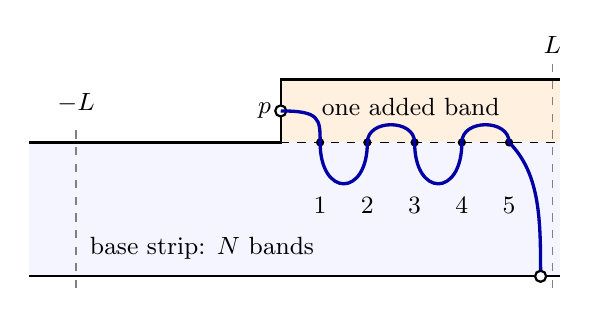
\begin{tikzpicture}[x=1cm,y=1cm,font=\small,>=Latex]
 \fill[blue!4] (-3.2,0) rectangle (3.55,1.7);
 \fill[orange!12] (0,1.7) rectangle (3.55,2.5);
 \draw[thick] (-3.2,0)--(3.55,0);
 \draw[thick] (-3.2,1.7)--(0,1.7)--(0,2.5)--(3.55,2.5);
 \draw[dashed] (0,1.7)--(3.55,1.7);
 \draw[black!50,dashed] (-2.6,-.15)--(-2.6,1.95);
 \draw[black!50,dashed] (3.45,-.15)--(3.45,2.7);
 \node[above] at (-2.6,1.95) {$-L$};
 \node[above] at (3.45,2.7) {$L$};
 \draw[fill=white,thick] (0,2.1) circle (2pt);
 \node[left] at (0,2.1) {$p$};
 \node at (-1.0,.35) {base strip: $N$ bands};
 \node at (1.65,2.15) {one added band};
 \foreach \x/\j in {.5/1,1.1/2,1.7/3,2.3/4,2.9/5}{
  \fill (\x,1.7) circle (1.5pt);
  \node at (\x,.9) {$\j$};
 }
 \draw[very thick,blue!65!black] (0,2.1) .. controls (.5,2.1) and (.5,2.0) .. (.5,1.7);
 \draw[very thick,blue!65!black] (.5,1.7) .. controls (.5,1.0) and (1.1,1.0) .. (1.1,1.7);
 \draw[very thick,blue!65!black] (1.1,1.7) .. controls (1.1,2.0) and (1.7,2.0) .. (1.7,1.7);
 \draw[very thick,blue!65!black] (1.7,1.7) .. controls (1.7,1.0) and (2.3,1.0) .. (2.3,1.7);
 \draw[very thick,blue!65!black] (2.3,1.7) .. controls (2.3,2.0) and (2.9,2.0) .. (2.9,1.7);
 \draw[very thick,blue!65!black] (2.9,1.7) .. controls (3.3,1.3) and (3.3,.7) .. (3.3,0);
 \draw[fill=white,thick] (3.3,0) circle (2pt);
\end{tikzpicture}
\caption{The stepped strip used to compare $m_{N+1}$ and $m_N$.
The drawing is schematic: curves represent path pieces, not individual
lattice edges. Interface visits are numbered from left to right.
A single connected path forces alternating consecutive pairings in the
added row and the base strip; the final visit connects to the bottom.
Moving the two dashed cuts to infinity recovers the two homogeneous
arch moments.}
\label{fig:stepped-strip}
\end{figure}


From a bottom source $i$, the imaginary
part of the boundary identity is
\begin{equation}\label{eq:01-step-identity}
 \sin(3\lambda)\left(
   \sum_{j<i}\overline K(i,j)-\sum_{j>i}\overline K(i,j)
 \right)+\sin\lambda\,Z(i,p)=0.
\end{equation}
Indeed horizontal top exits have winding zero, and closing along the
leftward boundary gives winding $\pi/3$ at $p$. Lateral truncation
errors vanish as before, dominated by a strip of height $N+1$.

Sum \eqref{eq:01-step-identity} over $-L\le i\le L$. Reversal pairs
and cancels all internal arches. The uncanceled terms cross the two
ends of this interval. After translating each end to the origin,
the stepped domains converge locally to strips of heights $N$ and
$N+1$, respectively. All crossing sums are dominated by the first
moment in the strip of height $N+1$, which is finite by transfer
decay. This also controls paths leaving an arbitrarily large lateral
window for each fixed pair of ports. Dominated convergence therefore
gives the exact identity
\begin{equation}\label{eq:01-step-moment}
 m_{N+1}-m_N=\frac{\sin\lambda}{\sin(3\lambda)}
                 \sum_i Z(p,i).
\end{equation}

Turning down immediately from $p$ and following an arbitrary bridge
in the base strip yields
$\sum_iZ(p,i)\ge\rho\mathcal B_N$. The top-source bridge mass in the
base strip equals its bottom-source mass by translation and reversal.

For the upper bound, order the path's visits to the interface between
the base strip and the new row from left to right. In the new row,
whose top is vacant, disjoint intervals pair $p$ with the first visit
and then pair subsequent visits consecutively. The base portions are
a noncrossing pairing with one unpaired visit connected to the bottom;
that defect cannot be enclosed. Since the union is a single path,
the first base visit must pair with its next neighbor: pairing it
farther away would leave a closed component inside. Removing these
two visits and repeating proves that base visits also pair
consecutively, with the last visit the defect. Thus the path encounters
the interface in increasing horizontal order.

At $u=\lambda$, the initial new-row segment has total weight at most
$A/(1-B)$. A one-sided base return arch has total mass at most
$1/(2c)$, using the boundary identity from the top and equality of
the two directions by translation and reversal. A one-sided return
through the new row has total mass
$AU/(1-B)=2cB$. The final base segment has total mass
$\mathcal B_N$. Ignoring avoidance between pieces only increases the
sum, since the base weights are products over vertices. Therefore
\[
 \sum_iZ(p,i)
 \le\frac{A}{1-B}\sum_{r\ge0}
       \left(\frac1{2c}\,2cB\right)^r\mathcal B_N
 =\frac{A}{(1-B)^2}\mathcal B_N.
\]
Here $B=B(\lambda)=\rho^2<1$, so the constants are independent of
$N$. Combine this with \eqref{eq:01-step-moment}.
\end{proof}

\section{A positive integral for the homogeneous moment}\label{sec:integral}

The arch formula \eqref{eq:01-arch-formula} is exact, but its Pfaffian
quotient does not directly show the size of $m_N$. We convert the
coalescing-parameter problem into a positive integral. This will establish
the limiting quotient without assuming that its denominator remains
nonzero, and make the moment accessible to comparison estimates.
For generic $X$, put $b=\cos w$ and
\begin{equation}\label{eq:01-Q-definition}
 \begin{split}
 Q_X(b)&=(b-C)g_X(b)\prod_{i=1}^N
  (b-a_i)(\cos(w-2\lambda)-a_i)(\cos(w+2\lambda)-a_i),\\
 \Phi_X(w)&=\sin w\,Q_X(\cos w).
 \end{split}
\end{equation}
The paired shifted factors have product
$b^2-2da_i b+a_i^2-d^2$, so $Q_X$ is a polynomial of degree $4N+1$.

\begin{lemma}[Missing harmonics]\label{lem:missing-harmonics}
Every sine harmonic of $\Phi_X$ whose frequency is divisible by four
has coefficient zero. Equivalently, writing
$h=b^2(1-b^2)=(1-\cos4w)/8$, there are polynomials such that
\begin{equation}\label{eq:01-projection}
 Q_X(b)=\mathcal P(h)+b\mathcal J(h)+b^2\mathcal E(h),
 \quad \deg\mathcal P,\deg\mathcal J\le N,
 \quad \deg\mathcal E\le N-1.
\end{equation}
\end{lemma}

\begin{proof}
Fix $i$ and write $f_j=\cos(v+j\lambda)$ with $f_0=a_i$.
The product in \eqref{eq:01-Q-definition} gives
$\Phi_X(v\pm2\lambda)=0$. The deletion quotient also gives
$\Phi_X(v+6\lambda)+\Phi_X(v-6\lambda)=0$. To verify its sign and
factors, cancel the contributions of the other $a_j$ in the ratio:
on both sides these contributions involve exactly
$f_6,f_{-6},f_4,f_{-4},-f_0$. The remaining expressions are
\[
 R_\pm=\sin(v\pm6\lambda)(f_{\pm6}-C)
       (f_0+f_{\pm6}+\rho)(f_{\pm6}-f_0)(f_{\pm4}-f_0).
\]
Product-to-sum and $\rho=2cd$ give
\[
 R_\pm=\cos(2v)(f_{\pm6}-C)
             \sin(v\pm3\lambda)(\cos(v\pm3\lambda)+d).
\]
The last two expressions after removing $\cos(2v)$ are trigonometric
polynomials of degree three. They have the same six zeros
$v=\pm3\lambda,\pm5\lambda,\pm7\lambda$ modulo $2\pi$, and
opposite values at zero; hence they are negatives of each other.
This proves the claimed cancellation as a polynomial identity,
including where canceled factors vanish.

Consider the sum of the four shifts of $\Phi_X$ by
$\pm2\lambda,\pm6\lambda$. On frequency $k$ its multiplier is
$4\cos(4k\lambda)\cos(2k\lambda)$, nonzero precisely when four divides
$k$. Its maximum frequency is $4N+2$. Dividing this shifted sum by
$\sin4w$ therefore gives a polynomial in $\cos4w$ of degree at most
$N-1$. The preceding identities give $N$ distinct roots, for generic
$a_i$, so it is zero. This proves the harmonic assertion.

Every polynomial in $b$ has a unique expression
$P_0(h)+bP_1(h)+b^2P_2(h)+b^3P_3(h)$, by repeatedly using
$b^4=b^2-h$. The first three terms, after multiplication by $\sin w$,
have no frequency divisible by four. For the last term use
\[
 \sin w\,b^3=\frac14\sin2w+\frac18\sin4w.
\]
Its projection onto multiples of four is
$\frac18\sin4w\,P_3((1-\cos4w)/8)$, so it vanishes only if $P_3=0$.
The degree bounds follow from $\deg Q_X=4N+1$.
\end{proof}

At the homogeneous parameters $a_i=C$, the paired factors in
\eqref{eq:01-Q-definition} become $(b-C)(b-c)$. Thus the desired
limiting monic polynomial is characterized by
\begin{equation}\label{eq:01-homogeneous-projection}
 Q(b)=(b-C)^{2N+1}(b-c)^N g(b)
     =\mathcal P(h)+b\mathcal J(h)+b^2\mathcal E(h),
 \qquad \deg g=N.
\end{equation}

\begin{lemma}[Nonsingularity and integral representation]
\label{lem:positive-integral}
The monic problem \eqref{eq:01-homogeneous-projection} has a unique
solution, which is the limit of $g_X$ as all $a_i\to C$.
Let
\begin{equation}\label{eq:01-omega}
 \omega(x)=\frac12\sqrt{\sqrt{\frac{1+x}{2x}}-1},\qquad 0<x<1,
\end{equation}
and let $(y_1,\ldots,y_N)$ have density proportional to
\begin{equation}\label{eq:01-positive-law}
 \prod_{i=1}^N\omega(y_i)
 \prod_{i<j}\frac{(y_j-y_i)^2}{y_i+y_j},
 \qquad 0<y_1<\cdots<y_N<1.
\end{equation}
Then
\begin{equation}\label{eq:01-moment-integral}
 m_N=\frac\eta\pi\int_0^1
  \left(1-\E\prod_{i=1}^N\frac{y_i-x}{y_i+x}\right)
  \frac{\omega(x)}x\,dx.
\end{equation}
\end{lemma}

\begin{proof}
We first turn the zero-multiplicity conditions into Cauchy-transform
moment equations. A positive determinant will make those equations
uniquely solvable and control the coalescing limit. We then identify the
resulting coefficient with the expectation in
\eqref{eq:01-moment-integral}.
The proposed probability law is well defined: $\omega(x)=O(x^{-1/4})$
at zero and each pair factor is at most $y_j\le1$, so its normalizing
integral is finite; it is positive because the density is positive
inside the ordered region.

\smallskip\noindent\emph{Cauchy moment equations.}
The two prescribed zeros satisfy $h(C)=h(c)=1/8$. To place them at
infinity, set $z=(8h-1)^{-1}$, so that the inverse relation is
\[
 b^2(1-b^2)=\frac{1+1/z}{8}.
\]
We use the two branches near infinity tending to $C$ and $c$, respectively.
Their differences from these limits have order $z^{-1}$, since
$h'(C)$ and $h'(c)$ are nonzero. For each polynomial in
\eqref{eq:01-homogeneous-projection}, multiply by $z^N$ after the
substitution $h=(1+1/z)/8$. Denote the resulting polynomials by
$\widetilde{\mathcal P}$, $\widetilde{\mathcal J}$, and
$\widetilde{\mathcal E}$; the last satisfies
$\widetilde{\mathcal E}(0)=0$ because $\deg\mathcal E\le N-1$.
The branch tending to $C$ and the sum of the two branches are, respectively,
\[
 f(z)=\sqrt{\frac{1+\sqrt{(1-1/z)/2}}2},\qquad
 l(z)=\sqrt{1+\sqrt{(1+1/z)/2}}.
\]
These formulas continue $f$ analytically off $[0,1]$ and $l$ off
$[-1,0]$. On the $C$ branch, the zero of order $2N+1$ in
\eqref{eq:01-homogeneous-projection} becomes $O(z^{-2N-1})$; on the
$c$ branch, the zero of order $N$ becomes $O(z^{-N})$.
After multiplication by $z^N$ this gives
\begin{align}
 \mathcal F(z)&=\widetilde{\mathcal P}(z)
        +f(z)\widetilde{\mathcal J}(z)
        +f(z)^2\widetilde{\mathcal E}(z)=O(z^{-N-1}),
        \label{eq:01-F-decay}\\
 \mathcal D(z)&=\widetilde{\mathcal J}(z)
                 +l(z)\widetilde{\mathcal E}(z)=O(1).
        \label{eq:01-D-decay}
\end{align}
For the second statement, evaluate the same polynomial expression
on the branch tending to $c$, where multiplication by $z^N$ makes
it $O(1)$, and subtract the expression on the $C$ branch; the
quotient by their nonzero difference is $\mathcal D$.

With subscripts $+$ and $-$ denoting boundary values from the upper
and lower half-planes, the jumps across the cuts are
\[
 f_+(x)-f_-(x)=2i\omega(x),\qquad
 l_+(-x)-l_-(-x)=-2\sqrt2\,i\omega(x),\qquad
 f_+(x)+f_-(x)=l(x).
\]
At the outer endpoints these functions are bounded. At zero,
$\mathcal F=O(|z|^{-1/4})$ and
$\mathcal D(z)\to D_0:=\widetilde{\mathcal J}(0)$;
the latter uses $\widetilde{\mathcal E}(0)=0$. Cauchy's formula,
with small endpoint circles shrinking to zero, yields
\begin{align}
 \mathcal F(z)&=\frac1\pi\int_0^1
                   \frac{\mathcal D(x)\omega(x)}{x-z}\,dx,
        \label{eq:01-F-Cauchy}\\
 \int_0^1x^j\mathcal D(x)\omega(x)\,dx&=0,
                  \qquad 0\le j<N,
        \label{eq:01-moments}\\
 \mathcal D(z)&=D_0-\frac{\sqrt2}{\pi}z
       \int_0^1\frac{\widetilde{\mathcal E}(-y)/y}{z+y}
                    \omega(y)\,dy.
        \label{eq:01-D-Cauchy}
\end{align}
The moment equations are the first $N$ coefficients of the expansion
of \eqref{eq:01-F-Cauchy} at infinity. To obtain
\eqref{eq:01-D-Cauchy}, subtract the bounded-at-infinity representation
at zero. Its integrand is integrable there because
$\widetilde{\mathcal E}(-y)/y$ is a polynomial.

To control the endpoint at zero, use $\omega(x)=O(x^{-1/4})$ and
$\widetilde{\mathcal E}(z)=O(z)$ near zero. The increment in
\eqref{eq:01-D-Cauchy}, split at $y=x$, is bounded by
\[
 C\left(\int_0^x y^{-1/4}\,dy
       +x\int_x^1y^{-5/4}\,dy\right)=O(x^{3/4}).
\]
This estimate will also justify the singular moment integral below.

\smallskip\noindent\emph{Nonsingularity and coalescence.}
The polynomial $\widetilde{\mathcal E}(-y)/y$ has degree at most
$N-1$, and the moment equations determine it uniquely from $D_0$.
Indeed the corresponding matrix, apart from nonzero scalar factors,
is
\begin{equation}\label{eq:01-moment-matrix}
 M_{jk}=\int_0^1\int_0^1
           \frac{x^{j+1}y^k}{x+y}\omega(x)\omega(y)\,dx\,dy,
           \qquad 0\le j,k<N.
\end{equation}
Its determinant is strictly positive. This is the Cauchy-bimoment
positivity argument used in
\cite[Theorem~2.1]{BertolaGekhtmanSzmigielski2010}; we give the finite
determinant calculation for the present weights. Expand the determinant and
antisymmetrize successively in the $x$ and $y$ variables. On the
ordered integration regions the integrand becomes the product of
two positive Vandermonde determinants, $\prod_i x_i$, positive
weights, and the Cauchy determinant
\[
 \det\left[\frac1{x_i+y_j}\right]
 =\frac{\prod_{i<j}(x_j-x_i)(y_j-y_i)}{\prod_{i,j}(x_i+y_j)}>0.
\]
For completeness this identity follows by multiplying through by the
denominator: the numerator is alternating in each family and has
exactly the degree of the two Vandermondes. The remaining constant
is one, recursively evaluating at $x_N=-y_N$.

Consider now a solution of the homogeneous linear problem for $g$,
so $\deg g\le N-1$. The coefficient of $b^{4N+1}$ in $Q$ is zero.
Since
\[
 [b^{4N+1}]Q=(-8)^N D_0,
\]
we obtain $D_0=0$. Positivity of \eqref{eq:01-moment-matrix} forces
$\widetilde{\mathcal E}=0$; then
\eqref{eq:01-D-Cauchy} gives $\widetilde{\mathcal J}=0$, and
\eqref{eq:01-F-decay} gives $\widetilde{\mathcal P}=0$. Thus $g=0$.
For the monic problem, write $g(b)=b^N+\sum_{r=0}^{N-1}\gamma_r b^r$.
The excluded $b^3P_3(h)$ part in the proof of
Lemma~\ref{lem:missing-harmonics} has $N$ coefficients. Requiring them
to vanish therefore gives an $N\times N$ linear system for
$(\gamma_0,\ldots,\gamma_{N-1})$, and the established injectivity
proves that this system is invertible at the homogeneous parameters.
This proves existence and uniqueness of $g$.
Apply the same coefficient conditions to \eqref{eq:01-Q-definition},
with $g_X$ replaced by a monic unknown polynomial. Their matrix and right side depend
polynomially on the $a_i$, through the displayed zero factors, and
converge to those of the homogeneous system. This coefficient matrix
is consequently invertible for all $a_i$ sufficiently close to $C$.
The generic $g_X$ satisfies that system by
Lemma~\ref{lem:missing-harmonics}, so it converges to $g$.
The moment itself is regular at the homogeneous point by
Lemma~\ref{lem:transfer-decay}.

\smallskip\noindent\emph{The moment coefficient and its expectation.}
For this monic solution $D_0=(-8)^{-N}$. Put
$G(z)=\mathcal D(z)/D_0$.
The leading coefficient computation also gives
$[b^{4N}]Q=(-8)^N\widetilde{\mathcal P}(0)$. Comparing this with the
product in \eqref{eq:01-homogeneous-projection} gives the coefficient
needed by the arch formula:
\[
 [b^{N-1}]g(b)=\frac{\widetilde{\mathcal P}(0)}{D_0}
                    +(2N+1)C+Nc.
\]
Substitution into \eqref{eq:physical-arch-coefficient}, using
$C=\eta(2C+c)$, yields the first equality below:
\begin{equation}\label{eq:01-moment-D}
 m_N=-\eta\left(C+\frac{\widetilde{\mathcal P}(0)}{D_0}\right)
     =\frac\eta\pi\int_0^1(1-G(x))\frac{\omega(x)}x\,dx.
\end{equation}
For the second equality, use
\[
 f(z)=C+\frac1\pi\int_0^1\frac{\omega(x)}{x-z}\,dx
\]
and subtract $D_0f$ from \eqref{eq:01-F-Cauchy}, then let $z\to0-$.
Equation \eqref{eq:01-D-Cauchy} gives
$\mathcal D(x)-D_0=O(x^{3/4})$, so the integrand after subtraction is $O(x^{-1/2})$ at zero.
This ensures integrability and justifies the limit. On the left, terms involving
$f(z)(\widetilde{\mathcal J}(z)-D_0)$ and
$f(z)^2\widetilde{\mathcal E}(z)$ tend to zero.

The moment equations now have a unique solution. It remains to
exhibit their probabilistic solution, thereby identifying $G$ with the
expectation in \eqref{eq:01-moment-integral}. Let $\mathcal W_n$ denote
the product in \eqref{eq:01-positive-law} with $n$ coordinates, viewed
on $(0,1)^n$ without the ordering constraint. We use its normalized
symmetric law for $n=N$. Partial fractions give
\[
 \prod_{i=1}^N\frac{y_i-x}{y_i+x}
 =1-x\sum_{i=1}^N\frac{\alpha_i}{x+y_i},
 \qquad
 \alpha_i=2\prod_{j\ne i}\frac{y_j+y_i}{y_j-y_i}.
\]
After multiplication by the density, the factors in $\alpha_i$
cancel one Vandermonde and all corresponding denominator factors.
Each canceled term is integrable: its remaining polynomial factors
and pair kernels are bounded on $(0,1)^N$, as is $x/(x+y_i)$, and
the one-variable weights are integrable.
Integrating over the other variables therefore gives a representation
$1-x\int_0^1P(y)\omega(y)/(x+y)\,dy$ with $\deg P\le N-1$.
Its moments against $x^k\omega(x)$ vanish for $k<N$. To see this,
adjoin $x$ as an $(N+1)$st variable and use the density identity
\[
 x^k\omega(x)\mathcal W_N(y_1,\ldots,y_N)
       \prod_{i=1}^N\frac{y_i-x}{y_i+x}
 =\frac{x^k\mathcal W_{N+1}(x,y_1,\ldots,y_N)}
          {\prod_{i=1}^N(y_i-x)}.
\]
The left side is absolutely integrable, since the product has modulus
at most one. Symmetrizing the right side in all $N+1$ variables gives
zero by the elementary interpolation identity
\[
 \sum_{r=0}^N\frac{z_r^k}{\prod_{j\ne r}(z_j-z_r)}=0,
 \qquad 0\le k<N.
\]
Thus the expectation has the same polynomial Cauchy representation
and vanishing moments as $G$. The uniqueness argument using
\eqref{eq:01-moment-matrix} now identifies this expectation with $G$.
Substitute into \eqref{eq:01-moment-D}.
\end{proof}

\section{The smallest coordinate and the strip exponent}\label{sec:hard-edge}

The positive integral reduces the growth of the arch moment to the coordinates nearest zero. We prove the required bounds by comparing with an explicitly normalized Bures--Laguerre density. The comparison is at the level of positive measures, so it also controls the possible sign changes in the product appearing inside the integral.


The integral formula immediately gives
\begin{equation}\label{eq:01-inverse-comparison}
 \E y_1^{-1/4}\lesssim m_N
 \lesssim\E\left(\sum_{i=1}^Ny_i^{-1}\right)^{1/4}.
\end{equation}
To verify both estimates pointwise, put
$R(x)=\prod_i(y_i-x)/(y_i+x)$. Since each factor lies in $[-1,1]$,
$1-R(x)\ge0$, and telescoping the product gives
\[
 1-R(x)\le2\min\left\{1,x\sum_i y_i^{-1}\right\}.
\]
For $y_1/3<x<y_1/2$, all factors are nonnegative and the first is at
most $1/2$, so $1-R(x)\ge1/2$. Finally,
$\omega(x)\lesssim x^{-1/4}$ on $(0,1)$ and
$\omega(x)\asymp x^{-1/4}$ on $(0,1/2)$. Integrating the lower bound
on the indicated interval and splitting the upper integral at
$x=(\sum_i y_i^{-1})^{-1}$ proves
\eqref{eq:01-inverse-comparison}.

The reference inverse-moment estimates below will contribute a factor
$N^{1/2}$. Scaling those coordinates by a factor of order $N^{-1}$
will contribute a further $N^{1/4}$, producing the required $N^{3/4}$
for the arch moment. We now prove both the reference estimates and the
comparison that permits this scaling.

For comparison we use the generalized Bures--Laguerre family
\cite{ForresterKieburg2016}, in ordered coordinates and with parameter
$a>0$, having density
\begin{equation}\label{eq:01-Laguerre-law}
 \frac1{Z_n(a)}\prod_{i=1}^n r_i^{a-1}e^{-r_i}
          \prod_{i<j}\frac{(r_j-r_i)^2}{r_i+r_j},
 \qquad 0<r_1<\cdots<r_n<\infty.
\end{equation}
Expectations and probabilities for this law will carry subscripts
$n,a$ when clarification is needed.
The exponent of the one-variable weight is $a-1$ in our convention;
thus our $a$ equals the parameter in \cite[equation~(1.5)]{ForresterKieburg2016}
plus one. Our ordered normalizer is the corresponding unordered integral
divided by $n!$.
The following association statement is the continuous MTP$_2$ principle
of Sarkar, for log-supermodular densities
\cite[Theorem 2.27]{Bogso2014}; see also
\cite[equation (3.5)]{FallatEtAl2017}. We give a direct conditioning
proof for the ordered pair kernel used here.

\begin{lemma}[Association and monotone comparison]\label{lem:association}
Let $I\subset(0,\infty)$ be an interval, let $n\ge1$, and let
$w_1,\ldots,w_n$ be positive smooth functions on $I$. Suppose
\[
 \prod_{i=1}^n w_i(x_i)\prod_{i<j}K(x_i,x_j),\qquad
 K(x,y)=\frac{(y-x)^2}{x+y},\qquad x_1<\cdots<x_n,\quad x_i\in I,
\]
has finite positive normalizing integral. Its probability law is
positively associated: increasing integrable functions have nonnegative
covariance whenever the covariance is defined. The assertion also
holds after truncation to a shorter common interval. Consequently,
a coordinatewise increasing likelihood ratio shifts the coordinates
upwards in stochastic order, and a decreasing one shifts them
downwards.
\end{lemma}

\begin{proof}
The mixed derivative of each pair contribution is
\[
 \frac{\partial^2}{\partial x\partial y}\log K(x,y)
 =\frac2{(y-x)^2}+\frac1{(x+y)^2}>0.
\]
We prove association by induction on the number of coordinates,
initially for bounded increasing functions. Conditional on the
largest coordinate $t$, the remaining coordinates have a law of the
same form on the shorter interval, with modified one-variable
factors. They are associated by induction. If $s<t$, the ratio of
the conditional density at $s$ to that at $t$, on the former support,
is coordinatewise decreasing by the mixed-derivative inequality.
Extended by zero where a coordinate exceeds $s$, it remains
decreasing on the latter support. Association for the conditional
law at $t$ shows that a decreasing likelihood tilt decreases every
increasing expectation. If the ratio is unbounded, first truncate
it and pass to the limit by monotone convergence. Thus the
conditional expectation of any increasing function of all the
coordinates increases with $t$.

The law of total covariance now has two nonnegative terms:
conditional covariance by induction, and covariance of the two
conditional expectations by the one-dimensional inequality
\[
 \operatorname{Cov}(F(T),G(T))
 =\frac12\E[(F(T)-F(T'))(G(T)-G(T'))]\ge0.
\]
Here $T'$ is an independent copy of $T$. This proves association;
truncation and integrable approximation extend the assertion to the
stated class. Finally for an increasing likelihood ratio $L$,
$\E[FL]/\E L\ge\E F$ for increasing $F$, and the reversed inequality
holds for decreasing $L$. This is the claimed stochastic comparison.
\end{proof}

The upper comparison will use $a=1/2$, and the lower comparison will
use $a=1$. To estimate the minimum for $a=1$, we will first need an
inverse-moment bound for $a=2$. The next lemma develops all three
estimates from the same normalizing integral.

\begin{lemma}[Laguerre normalization and coordinate bounds]
\label{lem:laguerre}
For fixed $a>0$ and every integer $n\ge1$,
\begin{equation}\label{eq:01-normalizer}
 Z_n(a)=\prod_{i=0}^{n-1}\Gamma(a+i)
             \prod_{0\le i<j<n}\frac{j-i}{2a+i+j}.
\end{equation}
There exist constants $K_a,C_a$, depending only on $a$, such that
$\Prob_{n,a}(r_n\le K_an)$ is bounded below by a positive constant
independent of $n$, and, with $D_k=ak+k(k-1)/2$,
\begin{equation}\label{eq:01-small-coordinate}
 \Prob_{n,a}(r_k<h)
 \le\min\left\{1,\left(\frac{C_a h n^2}{k^3}\right)^{D_k}\right\},
 \qquad h>0,\quad 1\le k\le n.
\end{equation}
In particular,
\begin{align}
 \E_{n,1/2}\left(\sum_i r_i^{-1}\right)^{1/4}
       &\lesssim n^{1/2},\label{eq:01-reference-upper}\\
 \E_{n,2}\sum_i r_i^{-1}&\lesssim n^2,
       \label{eq:01-reference-inverse}\\
 \E_{n,1}r_1^{-1/4}&\gtrsim n^{1/2}.
       \label{eq:01-reference-lower}
\end{align}
The constants in the last three bounds are absolute.
\end{lemma}

\begin{proof}
\emph{Normalization.}
Write the pair product as a Vandermonde determinant times the Schur
Pfaffian with entries $(s-r)/(s+r)$. The classical identity, in the
form recorded in \cite[equation (1.2)]{IshikawaOkadaTagawaZeng2006}, is
\[
 \operatorname{Pf}\left[\frac{x_j-x_i}{x_j+x_i}\right]
 =\prod_{i<j}\frac{x_j-x_i}{x_j+x_i}.
\]
For even size, clearing denominators leaves an alternating
polynomial of Vandermonde degree, so only its constant factor needs
checking. Pairing two opposite arguments gives that constant
recursively as one. For odd size, add an argument tending to infinity;
the resulting augmenting column consists of ones.

Expand the determinant and the Pfaffian and integrate over the
unordered region, divided by $n!$. This is de Bruijn's
determinant--Pfaffian integration formula~\cite{deBruijn1955}; the
general antisymmetric-kernel form, including its odd-size border,
is stated in \cite[Theorem 6.1]{BaikRains2001Algebraic}. The result is
the Pfaffian of double moments, with the single moments as augmenting
entries in odd size. Absolute integrability follows from
$|(s-r)/(s+r)|\le1$ and the finite gamma moments for $a>0$.
The double moment with indices $i,j$ is
\[
 \int_0^\infty\!\int_0^\infty
 r^{a+i-1}s^{a+j-1}e^{-r-s}\frac{s-r}{s+r}\,dr\,ds
 =\Gamma(a+i)\Gamma(a+j)\frac{j-i}{2a+i+j}.
\]
Use $r+s$ and $r/(r+s)$ to evaluate the integral; the latter beta
integral has mean $(a+i)/(2a+i+j)$. Factoring out the gamma terms and
using the Schur identity again, now at the arguments $a+i$, proves
\eqref{eq:01-normalizer}.

\smallskip\noindent\emph{Coordinate tails and inverse moments.}
For the maximum, condition on its value $s$. Every factor involving
a smaller coordinate is at most $s$, since $K(r,s)\le s$ for
$0<r<s$. Consequently
\[
 \Prob_{n,a}(r_n>Kn)
 \le\frac{Z_{n-1}(a)}{Z_n(a)}
         \int_{Kn}^\infty s^{a+n-2}e^{-s}\,ds.
\]
The explicit normalizer gives
\[
 \frac{Z_{n-1}(a)}{Z_n(a)}
 =\frac1{\Gamma(a+n-1)}
   \prod_{j=1}^{n-1}\frac{2a+2n-2-j}{j}
 \le\frac{e^a(2e)^{n-1}}{\Gamma(a+n-1)}.
\]
For $n\ge2$, the inequality follows by replacing every numerator by
$2(a+n-1)$, using $(n-1)!\ge((n-1)/e)^{n-1}$, and then
$(1+a/(n-1))^{n-1}\le e^a$; $n=1$ is immediate. The exponential-moment bound for a gamma random
variable gives
\[
 \frac1{\Gamma(a+n-1)}\int_{Kn}^\infty s^{a+n-2}e^{-s}\,ds
 \le e^{-Kn/2}2^{a+n-1}.
\]
Choosing $K$ large makes the desired tail uniformly small, and in
fact exponentially small in $n$.

For the small-coordinate estimate, integrate the first $k$
coordinates below $h$. Their mutual pair factors are at most $h$;
a factor between a small coordinate and a remaining one is at most
the latter. Discarding order constraints between these two groups
therefore gives
\begin{equation}\label{eq:01-small-normalizer-ratio}
 \Prob_{n,a}(r_k<h)
 \le\frac{h^{D_k}}{a^k k!}\frac{Z_{n-k}(a+k)}{Z_n(a)},
\end{equation}
with $Z_0=1$. From \eqref{eq:01-normalizer},
\[
 \frac{Z_{n-k}(a+k)}{Z_n(a)}
 =\prod_{i=0}^{k-1}\Gamma(a+i)^{-1}
  \prod_{\substack{0\le i<j<n\\i<k}}
       \left(1+\frac{2a+2i}{j-i}\right).
\]
For gaps $j-i\le k$, use $2a+2i\le C_a k$. For each $i<k$,
\[
 \sum_{j=1}^k\log(1+C_a k/j)
 \le k\log(1+C_a)+k\log k-\log(k!)=O_a(k).
\]
Thus the short gaps contribute $O_a(k^2)=O_a(D_k)$. For larger
gaps, $\log(1+x)\le x$ gives a contribution at most
\[
 \sum_{i<k}(2a+2i)\sum_{j=k+1}^{n-1-i}\frac1j
 \le 2D_k\log(n/k).
\]
This includes $k=n$, when all the latter sums are empty.
Furthermore
\begin{equation}\label{eq:01-gamma-product}
 \prod_{i=0}^{k-1}\Gamma(a+i)\ge k^{D_k}e^{-O_a(D_k)}.
\end{equation}
Here is a direct estimate. For $q=a+i$, integration on $[q,q+1]$
gives
$\log\Gamma(q)\ge(q-1)\log q-q-O_a(1)$.
Summing, separating the factor $\log k$, and using
$\sum_{i<k}(a+i)\log((a+i)/k)\ge-k^2/e$ gives
$D_k\log k-O_a(D_k)$; the missing $k\log k$ is absorbed in
$O_a(D_k)$. Adjust the constant for bounded $k$.
Combining these bounds with
\eqref{eq:01-small-normalizer-ratio}, and absorbing $a^{-k}/k!$
into $C_a^{D_k}$, proves \eqref{eq:01-small-coordinate}.

For any $0<p<D_k$, integration of that tail estimate gives
\begin{equation}\label{eq:01-inverse-tail}
 \E_{n,a}r_k^{-p}
 \le\frac{D_k}{D_k-p}
       \left(\frac{C_a n^2}{k^3}\right)^p.
\end{equation}
At $a=1/2$, apply this with $(k,p)=(1,1/4)$ and then with $p=1$,
$k\ge2$. It gives
$\E r_1^{-1/4}\lesssim n^{1/2}$ and
$\E\sum_{k\ge2}r_k^{-1}\lesssim n^2$.
Subadditivity of the fourth root and Jensen's inequality yield
\eqref{eq:01-reference-upper}. At $a=2$, use $p=1$ for every $k$
to obtain \eqref{eq:01-reference-inverse}.

\smallskip\noindent\emph{The minimum at $a=1$.}
The density of the smallest coordinate at $s>0$ is
\[
 e^{-s}\frac{Z_{n-1}(2)}{Z_n(1)}
 \E_{n-1,2}\left[
    \mathbf1_{\{r_i>s\ \forall i\}}
    \prod_i\frac{(1-s/r_i)^2}{1+s/r_i}\right].
\]
The normalizer ratio is exactly $n(n+1)/2$.
Set $q_s(r)=\mathbf1_{\{r>s\}}(1-s/r)^2/(1+s/r)$.
For all $r>0$, including $r\le s$, one has
$0\le q_s(r)\le1$ and $1-q_s(r)\le3s/r$. Consequently
\[
 \prod_iq_s(r_i)\ge1-3s\sum_i r_i^{-1}.
\]
By \eqref{eq:01-reference-inverse}, the expectation is at least
$1/2$ whenever $0<s<\varepsilon n^{-2}$ for a sufficiently small
fixed $\varepsilon>0$. The displayed density is then bounded below
by a positive multiple of $n^2$. An interval with endpoints fixed
positive multiples of $n^{-2}$ has probability bounded below;
on it $r_1^{-1/4}\gtrsim n^{1/2}$. This proves
\eqref{eq:01-reference-lower}, with $n=1$ also covered directly.
\end{proof}

\begin{proof}[Completion of Theorem~\ref{thm:strip}]
We compare \eqref{eq:01-positive-law} with the reference laws to
estimate the two sides of \eqref{eq:01-inverse-comparison}.
For the upper estimate, first condition the target law on
$y_N<1/2$. This decreasing event shifts all coordinates downwards,
by Lemma~\ref{lem:association}, and therefore increases the inverse
statistic. On this shorter interval compare it with
$y_i=r_i/(bN)$ under \eqref{eq:01-Laguerre-law} with $a=1/2$,
conditioned on $r_N<bN/2$. Up to a constant, the target-to-reference
likelihood ratio is the product of
\[
 \omega(y)y^{1/2}e^{bNy}.
\]
Direct differentiation gives
\[
 \frac{d}{dy}\log(\omega(y)y^{1/2})
 =\frac{1-2y-\sqrt{2y/(1+y)}}{4y(1-y)}\ge-4,
 \qquad 0<y\le\frac12.
\]
Indeed the numerator is positive for $y\le1/8$; on the remaining
interval it is at least $-1$ and the denominator is at least $1/4$.
Thus the likelihood factors are increasing for every $N\ge1$ once
$b\ge4$. Association shows that the conditioned reference
law has the larger inverse statistic. Choosing also $b/2\ge K_{1/2}$
makes its conditioning probability bounded below uniformly in $N$,
by Lemma~\ref{lem:laguerre}. Hence
\[
 \E\left(\sum_i y_i^{-1}\right)^{1/4}
 \lesssim (bN)^{1/4}
          \E_{N,1/2}\left(\sum_i r_i^{-1}\right)^{1/4}
 \lesssim N^{3/4}.
\]

For the lower estimate, set $y_i=2z_i/(1+z_i)$ in the target law,
so $0<z_1<\cdots<z_N<1$. The transformed pair kernel is
\[
 K\left(\frac{2z_i}{1+z_i},\frac{2z_j}{1+z_j}\right)
 =\frac{2K(z_i,z_j)}
 {(1+z_i)(1+z_j)(1+2z_iz_j/(z_i+z_j))}.
\]
Together with the Jacobian this gives one-variable factors
$\omega(2z/(1+z))(1+z)^{-(N+1)}$ and additional pair factors
$(1+2z_iz_j/(z_i+z_j))^{-1}$.
Compare with $z_i=r_i/(bN)$ under the reference law with $a=1$ and
fixed $0<b<1/2$, conditioned on $r_N<bN$. The ratio has individual
factors
\[
 \omega\left(\frac{2z}{1+z}\right)(1+z)^{-(N+1)}e^{bNz}
\]
and the additional pair factors just displayed. Each is decreasing
in every coordinate: $\omega$ is decreasing, and
$-(N+1)/(1+z)+bN<0$ for $0<z<1$. Association therefore puts the
target $z$ coordinates below those of this conditioned reference,
which are themselves below the unconditioned reference coordinates.
Since $y_1\le2z_1$, it follows that
\[
 \E y_1^{-1/4}
 \ge 2^{-1/4}(bN)^{1/4}\E_{N,1}r_1^{-1/4}
 \gtrsim N^{3/4}.
\]
Equation \eqref{eq:01-inverse-comparison} now proves
$m_N\asymp N^{3/4}$.

It remains to extract the bridge estimate from
Lemma~\ref{lem:moment-increments}. By monotonicity, summing the lower
increment bound over $1\le j<N$ gives
$(N-1)\mathcal B_N\lesssim m_N$, so
$\mathcal B_N\lesssim N^{-1/4}$, with bounded $N$ absorbed in the
constant. Conversely choose a fixed integer $L$ so large that the
lower bound for $m_{LN}$ exceeds twice the upper bound for $m_N$.
Then
\[
 N^{3/4}\lesssim m_{LN}-m_N
 \lesssim\sum_{j=N}^{LN-1}\mathcal B_j
 \le(L-1)N\mathcal B_N.
\]
This proves $\mathcal B_N\gtrsim N^{-1/4}$ and completes all assertions
of the theorem.
\end{proof}

\appendix
\section{Local coefficient identities}\label{app:local-calculations}
This appendix proves Lemma~\ref{lem:local-identities} in the diagram convention of Section~\ref{sec:flux}. The finite tables also specify every nonzero local coefficient used by the interpolation argument.

\begin{proof}
Equation \eqref{eq:01-factorization} follows by direct substitution.
For completeness we record a coefficient check of the splitting
identity. Subscripts $1,2$ mean arguments $x+s\lambda,x$. Let $q$ be
the cup coefficient and $k$ the strand coefficient of the splitter:
$q=k=\rho$ for $s=2$, and $q=1,k=0$ for $s=3$. Unsubscripted weights
refer to $\widehat R_s$; in the deletion case use $B=1$ and set its
other nonempty two-slot coefficients to zero. The inputs are the
passing auxiliary strand and the slot to be split; the latter is
absent in the deletion case. Outputs $1,2$ are the split slots and
output $3$ is the auxiliary slot. Input bits record occupancy. For one
input strand, a bare output index specifies its destination and a
parenthesized pair specifies an additional cup. The complete coefficient
check is
\[
\begin{array}{c|c|c|c}
\text{input}&\text{connections at output}&\text{left side}&(S_s\otimes I)\widehat R\\\hline
00&\emptyset&1&1\\
&12\ (\text{cup})& U_1 A_2+q B_1 B_2 &q\\
&13&U_1 B_2+q B_1 A_2 & k U\\
&23&U_2+q A_1 E_2&k U\\\hline
10&1&A_1+q F_1 U_2 & k A\\
&2&B_1 A_2+q U_1 B_2 &k A\\
&3&B_1 B_2+q U_1 A_2 & B\\
&3,(12)&q F_1 E_2 &q B\\
&1,(23)&A_1 U_2+q(E_1 E_2+F_1 F_2)&0
\end{array}
\]
\begin{samepage}
For $s=2$ there are also the following inputs. In the final $11$ block,
an empty output or a parenthesized output pair connects the two input
strands to one another; a bare pair of output indices denotes two
through-strands.
\[
\begin{array}{c|c|c|c}
01&1&k(B_1+U_1 U_2)& k B\\
&2&k(A_1 A_2+B_2)& k B\\
&3&k(A_1 B_2+A_2)& A\\
&1,(23)& k(B_1 U_2+U_1 F_2)&0\\
&3,(12)& k U_1 E_2 & q A\\\hline
11&\emptyset&k(U_1+B_1 U_2)& U\\
&12& k(E_1 A_2+A_1 B_2)&0\\
&(12)& k F_1 A_2 &q U\\
&13& k(E_1 B_2+A_1 A_2)& k E\\
&(13)& k F_1 B_2&k F\\
&23& k B_1 E_2&k E\\
&(23)&k(U_1 U_2+B_1 F_2)& k F
\end{array}
\]
\end{samepage}
Here are the substitutions verifying these equalities. Put
$s_j=\sin(x+j\lambda)$. The weights at $x+j\lambda$ have common
denominator $s_{j+2}s_{j+3}$ and numerators
\[
\begin{array}{c|ccccc}
\text{weight}&A&B&U&E&F\\\hline
\text{numerator}&d s_{j+5}&s_j s_{j+5}&d s_j&
 s_{j+5}s_{j+6}&-s_{j+7}s_j
\end{array}
\]
Substitution uses the following product-to-sum identities:
\[
\begin{gathered}
s_{j+8}=-s_j,\quad s_j s_{j+1}+s_{j+4}s_{j+5}=C,\quad
s_2s_6=d^2-s_0^2,\quad s_1s_5=d^2-s_7^2,\\
\rho(s_1-s_7)=s_0,\quad \rho(s_6-s_0)=s_7,\quad
\rho(s_1s_2-s_6s_7)=s_0s_4,\quad \rho(s_5s_6-s_0s_1)=s_7s_3,\\
\rho(s_7s_0+s_4s_5)=s_6s_2,\quad \rho(s_2s_3+s_7s_0)=s_1s_5,\quad
s_1s_6-s_7s_0=\rho d^2,\\
s_1s_6s_5=s_7s_2s_3+d^2s_0,\qquad s_1s_6s_2=s_0s_4s_5+d^2s_7
\end{gathered}
\]
The last two trigonometric identities also follow from the preceding
formulas for $s_1s_5$ and $s_6s_2$. Thus substitution verifies every
entry in the tables.

For \eqref{eq:01-unitarity}, the sector with one strand reduces to
multiplication of two matrices with diagonal entries $A$ and
off-diagonal entries $B$. In the even sector the required identities
are
\[
 E(x)E(-x)=1,\qquad U(x)+E(x)U(-x)=0,
\]
\[
 E(x)F(-x)+F(x)E(-x)+U(x)U(-x)=0.
\]
A cap composed with a cup creates a loop and therefore vanishes.
These identities again follow from \eqref{eq:01-rhombic-weights}.

To prove \eqref{eq:01-braid}, first set $y=s\lambda$, $s=2,3$.
Use \eqref{eq:01-factorization} and \eqref{eq:01-splitting}, together
with their transposes and the reversal of slot order. The effective
box is symmetric, and both sides become
$(I\otimes S_s)\widehat R_s(x)(S_s^{\mathsf t}\otimes I)$.
Unitarity transports these identities to $x+y=s\lambda$, by applying
the identity with arguments $(-x,x+y)$. The case $y=0$ follows from
$R(0)=I$.

Multiply the difference of the two sides by their three scalar
denominators, and call the resulting diagram sum $\mathcal F(x,y)$.
Each coefficient is a Laurent polynomial in $e^{iy}$ with exponents
between $-4$ and $4$. To see its parity, let $D_j$ multiply a diagram
by $-1$ when slot $j$ is occupied. Inspection of the nine boxes gives
\[
 R_i(v+\pi)=D_{i+1}R_i(v)D_i.
\]
On either side of the braid relation the two internal $D_2$ signs
cancel. The remaining signs are at input slot $1$ and output slot $3$;
the scalar denominators are $\pi$-periodic. Hence
\[
 \mathcal F(x,y+\pi)=D_3\mathcal F(x,y)D_1.
\]
Every boundary coefficient has fixed parity. After multiplication by
a Laurent monomial it is a polynomial of degree at most four in
$e^{2iy}$. We have proved its vanishing at
$y=0,2\lambda,3\lambda,2\lambda-x,3\lambda-x$; these five values
are distinct modulo $\pi$ for generic $x$. Interpolation proves the
identity, and rational continuation removes the genericity restriction.
\end{proof}

\begin{thebibliography}{99}
\bibitem{BaikRains2001Algebraic}
J.~Baik and E.~M.~Rains.
Algebraic aspects of increasing subsequences.
\emph{Duke Mathematical Journal} \textbf{109} (2001), 1--65.
\href{https://doi.org/10.1215/S0012-7094-01-10911-3}{doi:10.1215/S0012-7094-01-10911-3}.
\href{https://arxiv.org/abs/math/9905083}{arXiv:math/9905083}.

\bibitem{BeatonEtAl2014}
N.~R.~Beaton, M.~Bousquet-M\'elou, J.~de Gier, H.~Duminil-Copin and A.~J.~Guttmann.
The critical fugacity for surface adsorption of self-avoiding walks on the honeycomb lattice is $1+\sqrt2$.
\emph{Communications in Mathematical Physics} \textbf{326} (2014), 727--754.
\href{https://doi.org/10.1007/s00220-014-1896-1}{doi:10.1007/s00220-014-1896-1}.

\bibitem{BertolaGekhtmanSzmigielski2010}
M.~Bertola, M.~Gekhtman and J.~Szmigielski.
Cauchy biorthogonal polynomials.
\emph{Journal of Approximation Theory} \textbf{162} (2010), 832--867.
\href{https://doi.org/10.1016/j.jat.2009.09.008}{doi:10.1016/j.jat.2009.09.008}.
\href{https://arxiv.org/abs/0904.2602}{arXiv:0904.2602}.

\bibitem{Bogso2014}
A.~M.~Bogso.
An application of multivariate total positivity to peacocks.
\emph{ESAIM: Probability and Statistics} \textbf{18} (2014), 514--540.
\href{https://doi.org/10.1051/ps/2013049}{doi:10.1051/ps/2013049}.

\bibitem{deBruijn1955}
N.~G.~de Bruijn.
On some multiple integrals involving determinants.
\emph{Journal of the Indian Mathematical Society}, New Series,
\textbf{19} (1955), 133--151.
\href{https://pure.tue.nl/ws/files/1920642/597510.pdf}{Published article scan}.

\bibitem{DeGierNienhuisPonsaing2010}
J.~de Gier, B.~Nienhuis and A.~Ponsaing.
Exact spin quantum Hall current between boundaries of a lattice strip.
\emph{Nuclear Physics B} \textbf{838} (2010), 371--390.
\href{https://doi.org/10.1016/j.nuclphysb.2010.05.019}{doi:10.1016/j.nuclphysb.2010.05.019}.
\href{https://arxiv.org/abs/1004.4037v2}{arXiv:1004.4037v2}.

\bibitem{DiFrancesco2005Open}
P.~Di Francesco.
Inhomogeneous loop models with open boundaries.
\emph{Journal of Physics A: Mathematical and General} \textbf{38} (2005), 6091--6120.
\href{https://doi.org/10.1088/0305-4470/38/27/001}{doi:10.1088/0305-4470/38/27/001}.
\href{https://arxiv.org/abs/math-ph/0504032v2}{arXiv:math-ph/0504032v2}.

\bibitem{DiFrancescoZinnJustin2005}
P.~Di Francesco and P.~Zinn-Justin.
Around the Razumov--Stroganov conjecture: proof of a multi-parameter sum rule.
\emph{Electronic Journal of Combinatorics} \textbf{12} (2005), Research Paper~6.
\href{https://doi.org/10.37236/1903}{doi:10.37236/1903}.
\href{https://arxiv.org/abs/math-ph/0410061}{arXiv:math-ph/0410061}.

\bibitem{DCS2012}
H.~Duminil-Copin and S.~Smirnov.
The connective constant of the honeycomb lattice equals $\sqrt{2+\sqrt2}$.
\emph{Annals of Mathematics} \textbf{175} (2012), 1653--1665.
\href{https://doi.org/10.4007/annals.2012.175.3.14}{doi:10.4007/annals.2012.175.3.14}.

\bibitem{FallatEtAl2017}
S.~Fallat, S.~Lauritzen, K.~Sadeghi, C.~Uhler, N.~Wermuth and P.~Zwiernik.
Total positivity in Markov structures.
\emph{Annals of Statistics} \textbf{45} (2017), 1152--1184.
\href{https://doi.org/10.1214/16-AOS1478}{doi:10.1214/16-AOS1478}.

\bibitem{FeherNienhuis2018}
G.~Z.~Feh\'er and B.~Nienhuis.
Currents in the dilute $O(n=1)$ model.
Preprint, 2015; revised November~7, 2018.
\href{https://arxiv.org/abs/1510.02721v2}{arXiv:1510.02721v2}.

\bibitem{ForresterKieburg2016}
P.~J.~Forrester and M.~Kieburg.
Relating the Bures measure to the Cauchy two-matrix model.
\emph{Communications in Mathematical Physics} \textbf{342} (2016), 151--187.
\href{https://doi.org/10.1007/s00220-015-2435-4}{doi:10.1007/s00220-015-2435-4}.
\href{https://arxiv.org/abs/1410.6883}{arXiv:1410.6883}.

\bibitem{GarbaliNienhuis2017Ground}
A.~Garbali and B.~Nienhuis.
The dilute Temperley--Lieb $O(n=1)$ loop model on a semi infinite strip:
the ground state.
\emph{Journal of Statistical Mechanics: Theory and Experiment} (2017), 043108.
\href{https://doi.org/10.1088/1742-5468/aa6a30}{doi:10.1088/1742-5468/aa6a30}.
\href{https://arxiv.org/abs/1411.7020}{arXiv:1411.7020}.

\bibitem{GarbaliNienhuis2017Sum}
A.~Garbali and B.~Nienhuis.
The dilute Temperley--Lieb $O(n=1)$ loop model on a semi infinite strip:
the sum rule.
\emph{Journal of Statistical Mechanics: Theory and Experiment} (2017), 053102.
\href{https://doi.org/10.1088/1742-5468/aa6bc3}{doi:10.1088/1742-5468/aa6bc3}.
\href{https://arxiv.org/abs/1411.7160}{arXiv:1411.7160}.

\bibitem{Glazman2015}
A.~Glazman.
Connective constant for a weighted self-avoiding walk on $\mathbb Z^2$.
\emph{Electronic Communications in Probability} \textbf{20} (2015), paper 86, 1--13.
\href{https://doi.org/10.1214/ECP.v20-3844}{doi:10.1214/ECP.v20-3844}.

\bibitem{GM2019}
A.~Glazman and I.~Manolescu.
Self-avoiding walk on $\mathbb Z^2$ with Yang--Baxter weights: universality of critical fugacity and 2-point function.
\emph{Annales de l'Institut Henri Poincar\'e, Probabilit\'es et Statistiques}
\textbf{56} (2020), 2281--2300.
\href{https://doi.org/10.1214/19-AIHP1024}{doi:10.1214/19-AIHP1024}.

\bibitem{GrimmPearce1993}
U.~Grimm and P.~A.~Pearce.
Multi-colour braid--monoid algebras.
\emph{Journal of Physics A: Mathematical and General} \textbf{26} (1993), 7435--7460.
\href{https://doi.org/10.1088/0305-4470/26/24/018}{doi:10.1088/0305-4470/26/24/018}.
\href{https://arxiv.org/abs/hep-th/9303161}{arXiv:hep-th/9303161}.

\bibitem{IkhlefCardy2009}
Y.~Ikhlef and J.~Cardy.
Discretely holomorphic parafermions and integrable loop models.
\emph{Journal of Physics A: Mathematical and Theoretical} \textbf{42} (2009), 102001.
\href{https://doi.org/10.1088/1751-8113/42/10/102001}{doi:10.1088/1751-8113/42/10/102001}.

\bibitem{IshikawaOkadaTagawaZeng2006}
M.~Ishikawa, S.~Okada, H.~Tagawa and J.~Zeng.
Generalizations of Cauchy's determinant and Schur's Pfaffian.
\emph{Advances in Applied Mathematics} \textbf{36} (2006), 251--287.
\href{https://doi.org/10.1016/j.aam.2005.07.001}{doi:10.1016/j.aam.2005.07.001}.
\href{https://arxiv.org/abs/math/0411280}{arXiv:math/0411280}.

\bibitem{KrachunPanagiotis2026}
D.~Krachun and C.~Panagiotis.
Quantitative sub-ballisticity of self-avoiding walk on the hexagonal lattice.
\emph{Annals of Probability} \textbf{54} (2026), 1109--1125.
\href{https://doi.org/10.1214/24-AOP1730}{doi:10.1214/24-AOP1730}.
\href{https://arxiv.org/abs/2310.17299}{arXiv:2310.17299}.

\bibitem{LawlerSchrammWerner2004}
G.~F.~Lawler, O.~Schramm and W.~Werner.
On the scaling limit of planar self-avoiding walk.
In \emph{Fractal Geometry and Applications: A Jubilee of Beno\^it Mandelbrot},
Part~2, Proceedings of Symposia in Pure Mathematics \textbf{72},
American Mathematical Society, Providence, RI, 2004, 339--364.
\href{https://arxiv.org/abs/math/0204277v2}{arXiv:math/0204277v2}.

\bibitem{Nienhuis1982}
B.~Nienhuis.
Exact critical point and critical exponents of $O(n)$ models in two dimensions.
\emph{Physical Review Letters} \textbf{49} (1982), 1062--1065.
\href{https://doi.org/10.1103/PhysRevLett.49.1062}{doi:10.1103/PhysRevLett.49.1062}.

\bibitem{Nienhuis1990CriticalMulticritical}
B.~Nienhuis.
Critical and multicritical $O(n)$ models.
\emph{Physica A} \textbf{163} (1990), 152--157.
\href{https://doi.org/10.1016/0378-4371(90)90325-M}{doi:10.1016/0378-4371(90)90325-M}.
\end{thebibliography}

\end{document}
